\documentclass[11pt]{article}

% Shared notes settings for Applied Machine Learning lectures (UPES).
% Keep this file free of \documentclass to allow reuse via \input.

\usepackage[utf8]{inputenc}
\usepackage[T1]{fontenc}
\usepackage{lmodern}          % scalable T1 fonts; without this pdflatex falls back
\input{glyphtounicode}        % to bitmapped EC Type 3 and the PDFs are neither
\pdfgentounicode=1            % searchable nor screen-reader friendly
\usepackage[a4paper,margin=1in]{geometry}
\usepackage{hyperref}
\usepackage{xurl}
\usepackage{booktabs}
\usepackage{amsmath}
\usepackage{amssymb}
\usepackage{listings}
\usepackage{xcolor}
\usepackage{enumitem}
\usepackage{parskip}

% Code listings (Python-oriented for this subject).
\lstset{
  language=Python,
  basicstyle=\ttfamily\small,
  keywordstyle=\color{blue},
  commentstyle=\color{gray},
  stringstyle=\color{teal},
  showstringspaces=false,
  columns=fullflexible,
  frame=single,
  framerule=0.2pt,
  breaklines=true
}

\setlist[itemize]{topsep=0.3em,itemsep=0.2em}
\setlist[enumerate]{topsep=0.3em,itemsep=0.2em}

% Simple per-section source line.
\newcommand{\notesources}[1]{\par\noindent{\small\color{gray}\textit{Sources:} \sloppy #1\par}}

% Unit-wise source strings for this subject (used by slides + notes).
% Path is relative to the lecture `latex/` folder (the compilation CWD).
\IfFileExists{../../../_shared/aml-sources.tex}{%
  % Source strings for Applied Machine Learning (CSAI2017P) — used by slides + notes.
% Prescribed texts and reference books are taken from the course syllabus.
% Support texts are the author-hosted open-access editions:
%   statlearning.com            (ISL with Python)
%   probml.github.io/pml-book   (Murphy, Probabilistic Machine Learning)
%   d2l.ai                      (Dive into Deep Learning)
%   mml-book.github.io          (Mathematics for Machine Learning)

\newcommand{\AMLRepoURL}{https://github.com/tali7c/Applied-Machine-Learning}

% --- prescribed -------------------------------------------------------------
\newcommand{\AMLPrescribed}{%
M\"uller and Guido, \textit{Introduction to Machine Learning with Python}, O'Reilly, 2016.;%
Bishop, \textit{Pattern Recognition and Machine Learning}, Springer, 2006.;%
Murphy, \textit{Machine Learning: A Probabilistic Perspective}, MIT Press, 2012.;%
Han, Kamber and Pei, \textit{Data Mining: Concepts and Techniques} (3e), Morgan Kaufmann, 2012.%
}

% --- unit-wise ---------------------------------------------------------------
\newcommand{\AMLUnitISources}{%
M\"uller and Guido, \textit{Introduction to Machine Learning with Python}, Ch. 1.;%
Bishop, \textit{Pattern Recognition and Machine Learning}, Ch. 1.;%
Murphy, \textit{Probabilistic Machine Learning: An Introduction}, MIT Press, 2022, Ch. 1.;%
Mitchell, \textit{Machine Learning}, McGraw Hill, 1997, Ch. 1.;%
Scikit-learn documentation, accessed 2026-08-04.%
}

\newcommand{\AMLUnitIISources}{%
Bishop, \textit{Pattern Recognition and Machine Learning}, \S1.5, \S4.3, \S7.1.;%
Zhang, Lipton, Li and Smola, \textit{Dive into Deep Learning}, \S3.4.;%
Shalev-Shwartz and Ben-David, \textit{Understanding Machine Learning}, Ch. 15.;%
Murphy, \textit{Probabilistic Machine Learning: An Introduction}, Ch. 5.%
}

\newcommand{\AMLUnitIIISources}{%
Zhang, Lipton, Li and Smola, \textit{Dive into Deep Learning}, Ch. 12 (Optimization Algorithms).;%
Deisenroth, Faisal and Ong, \textit{Mathematics for Machine Learning}, Ch. 7.;%
Kingma and Ba, ``Adam: A Method for Stochastic Optimization,'' ICLR 2015.;%
Ruder, ``An overview of gradient descent optimization algorithms,'' arXiv:1609.04747, 2016.%
}

\newcommand{\AMLUnitIVSources}{%
Han, Kamber and Pei, \textit{Data Mining: Concepts and Techniques} (3e), Ch. 3.;%
M\"uller and Guido, \textit{Introduction to Machine Learning with Python}, Ch. 3--4.;%
James, Witten, Hastie, Tibshirani and Taylor, \textit{An Introduction to Statistical Learning with Python}, Ch. 5--6, 12.;%
Scikit-learn documentation (preprocessing, model selection), accessed 2026-08-04.%
}

\newcommand{\AMLUnitVSources}{%
James et al., \textit{An Introduction to Statistical Learning with Python}, Ch. 3--6.;%
Bishop, \textit{Pattern Recognition and Machine Learning}, Ch. 3.;%
Deisenroth, Faisal and Ong, \textit{Mathematics for Machine Learning}, Ch. 9.;%
M\"uller and Guido, \textit{Introduction to Machine Learning with Python}, \S2.3.%
}

\newcommand{\AMLUnitVISources}{%
Han, Kamber and Pei, \textit{Data Mining: Concepts and Techniques} (3e), Ch. 8--9.;%
James et al., \textit{An Introduction to Statistical Learning with Python}, Ch. 8--9.;%
Bishop, \textit{Pattern Recognition and Machine Learning}, Ch. 4--5, 7, 14.;%
Zhang et al., \textit{Dive into Deep Learning}, Ch. 5.%
}

\newcommand{\AMLUnitVIISources}{%
Han, Kamber and Pei, \textit{Data Mining: Concepts and Techniques} (3e), Ch. 10.;%
James et al., \textit{An Introduction to Statistical Learning with Python}, Ch. 12.;%
M\"uller and Guido, \textit{Introduction to Machine Learning with Python}, \S3.5.;%
Ester, Kriegel, Sander and Xu, ``A density-based algorithm for discovering clusters (DBSCAN),'' KDD 1996.%
}

\newcommand{\AMLLabSources}{%
M\"uller and Guido, \textit{Introduction to Machine Learning with Python}, companion notebooks.;%
McKinney, \textit{Python for Data Analysis} (3e), O'Reilly, 2022.;%
Scikit-learn user guide, accessed 2026-08-04.;%
Matplotlib and Seaborn documentation, accessed 2026-08-04.%
}
%
}{%
  % Faculty copies live under `private/` so their compile CWD is different.
  \IfFileExists{../../../../public/_shared/aml-sources.tex}{%
    % Source strings for Applied Machine Learning (CSAI2017P) — used by slides + notes.
% Prescribed texts and reference books are taken from the course syllabus.
% Support texts are the author-hosted open-access editions:
%   statlearning.com            (ISL with Python)
%   probml.github.io/pml-book   (Murphy, Probabilistic Machine Learning)
%   d2l.ai                      (Dive into Deep Learning)
%   mml-book.github.io          (Mathematics for Machine Learning)

\newcommand{\AMLRepoURL}{https://github.com/tali7c/Applied-Machine-Learning}

% --- prescribed -------------------------------------------------------------
\newcommand{\AMLPrescribed}{%
M\"uller and Guido, \textit{Introduction to Machine Learning with Python}, O'Reilly, 2016.;%
Bishop, \textit{Pattern Recognition and Machine Learning}, Springer, 2006.;%
Murphy, \textit{Machine Learning: A Probabilistic Perspective}, MIT Press, 2012.;%
Han, Kamber and Pei, \textit{Data Mining: Concepts and Techniques} (3e), Morgan Kaufmann, 2012.%
}

% --- unit-wise ---------------------------------------------------------------
\newcommand{\AMLUnitISources}{%
M\"uller and Guido, \textit{Introduction to Machine Learning with Python}, Ch. 1.;%
Bishop, \textit{Pattern Recognition and Machine Learning}, Ch. 1.;%
Murphy, \textit{Probabilistic Machine Learning: An Introduction}, MIT Press, 2022, Ch. 1.;%
Mitchell, \textit{Machine Learning}, McGraw Hill, 1997, Ch. 1.;%
Scikit-learn documentation, accessed 2026-08-04.%
}

\newcommand{\AMLUnitIISources}{%
Bishop, \textit{Pattern Recognition and Machine Learning}, \S1.5, \S4.3, \S7.1.;%
Zhang, Lipton, Li and Smola, \textit{Dive into Deep Learning}, \S3.4.;%
Shalev-Shwartz and Ben-David, \textit{Understanding Machine Learning}, Ch. 15.;%
Murphy, \textit{Probabilistic Machine Learning: An Introduction}, Ch. 5.%
}

\newcommand{\AMLUnitIIISources}{%
Zhang, Lipton, Li and Smola, \textit{Dive into Deep Learning}, Ch. 12 (Optimization Algorithms).;%
Deisenroth, Faisal and Ong, \textit{Mathematics for Machine Learning}, Ch. 7.;%
Kingma and Ba, ``Adam: A Method for Stochastic Optimization,'' ICLR 2015.;%
Ruder, ``An overview of gradient descent optimization algorithms,'' arXiv:1609.04747, 2016.%
}

\newcommand{\AMLUnitIVSources}{%
Han, Kamber and Pei, \textit{Data Mining: Concepts and Techniques} (3e), Ch. 3.;%
M\"uller and Guido, \textit{Introduction to Machine Learning with Python}, Ch. 3--4.;%
James, Witten, Hastie, Tibshirani and Taylor, \textit{An Introduction to Statistical Learning with Python}, Ch. 5--6, 12.;%
Scikit-learn documentation (preprocessing, model selection), accessed 2026-08-04.%
}

\newcommand{\AMLUnitVSources}{%
James et al., \textit{An Introduction to Statistical Learning with Python}, Ch. 3--6.;%
Bishop, \textit{Pattern Recognition and Machine Learning}, Ch. 3.;%
Deisenroth, Faisal and Ong, \textit{Mathematics for Machine Learning}, Ch. 9.;%
M\"uller and Guido, \textit{Introduction to Machine Learning with Python}, \S2.3.%
}

\newcommand{\AMLUnitVISources}{%
Han, Kamber and Pei, \textit{Data Mining: Concepts and Techniques} (3e), Ch. 8--9.;%
James et al., \textit{An Introduction to Statistical Learning with Python}, Ch. 8--9.;%
Bishop, \textit{Pattern Recognition and Machine Learning}, Ch. 4--5, 7, 14.;%
Zhang et al., \textit{Dive into Deep Learning}, Ch. 5.%
}

\newcommand{\AMLUnitVIISources}{%
Han, Kamber and Pei, \textit{Data Mining: Concepts and Techniques} (3e), Ch. 10.;%
James et al., \textit{An Introduction to Statistical Learning with Python}, Ch. 12.;%
M\"uller and Guido, \textit{Introduction to Machine Learning with Python}, \S3.5.;%
Ester, Kriegel, Sander and Xu, ``A density-based algorithm for discovering clusters (DBSCAN),'' KDD 1996.%
}

\newcommand{\AMLLabSources}{%
M\"uller and Guido, \textit{Introduction to Machine Learning with Python}, companion notebooks.;%
McKinney, \textit{Python for Data Analysis} (3e), O'Reilly, 2022.;%
Scikit-learn user guide, accessed 2026-08-04.;%
Matplotlib and Seaborn documentation, accessed 2026-08-04.%
}
%
  }{%
    % Question papers live at `private/<family>/<instrument>/`.
    \IfFileExists{../../../public/_shared/aml-sources.tex}{%
      % Source strings for Applied Machine Learning (CSAI2017P) — used by slides + notes.
% Prescribed texts and reference books are taken from the course syllabus.
% Support texts are the author-hosted open-access editions:
%   statlearning.com            (ISL with Python)
%   probml.github.io/pml-book   (Murphy, Probabilistic Machine Learning)
%   d2l.ai                      (Dive into Deep Learning)
%   mml-book.github.io          (Mathematics for Machine Learning)

\newcommand{\AMLRepoURL}{https://github.com/tali7c/Applied-Machine-Learning}

% --- prescribed -------------------------------------------------------------
\newcommand{\AMLPrescribed}{%
M\"uller and Guido, \textit{Introduction to Machine Learning with Python}, O'Reilly, 2016.;%
Bishop, \textit{Pattern Recognition and Machine Learning}, Springer, 2006.;%
Murphy, \textit{Machine Learning: A Probabilistic Perspective}, MIT Press, 2012.;%
Han, Kamber and Pei, \textit{Data Mining: Concepts and Techniques} (3e), Morgan Kaufmann, 2012.%
}

% --- unit-wise ---------------------------------------------------------------
\newcommand{\AMLUnitISources}{%
M\"uller and Guido, \textit{Introduction to Machine Learning with Python}, Ch. 1.;%
Bishop, \textit{Pattern Recognition and Machine Learning}, Ch. 1.;%
Murphy, \textit{Probabilistic Machine Learning: An Introduction}, MIT Press, 2022, Ch. 1.;%
Mitchell, \textit{Machine Learning}, McGraw Hill, 1997, Ch. 1.;%
Scikit-learn documentation, accessed 2026-08-04.%
}

\newcommand{\AMLUnitIISources}{%
Bishop, \textit{Pattern Recognition and Machine Learning}, \S1.5, \S4.3, \S7.1.;%
Zhang, Lipton, Li and Smola, \textit{Dive into Deep Learning}, \S3.4.;%
Shalev-Shwartz and Ben-David, \textit{Understanding Machine Learning}, Ch. 15.;%
Murphy, \textit{Probabilistic Machine Learning: An Introduction}, Ch. 5.%
}

\newcommand{\AMLUnitIIISources}{%
Zhang, Lipton, Li and Smola, \textit{Dive into Deep Learning}, Ch. 12 (Optimization Algorithms).;%
Deisenroth, Faisal and Ong, \textit{Mathematics for Machine Learning}, Ch. 7.;%
Kingma and Ba, ``Adam: A Method for Stochastic Optimization,'' ICLR 2015.;%
Ruder, ``An overview of gradient descent optimization algorithms,'' arXiv:1609.04747, 2016.%
}

\newcommand{\AMLUnitIVSources}{%
Han, Kamber and Pei, \textit{Data Mining: Concepts and Techniques} (3e), Ch. 3.;%
M\"uller and Guido, \textit{Introduction to Machine Learning with Python}, Ch. 3--4.;%
James, Witten, Hastie, Tibshirani and Taylor, \textit{An Introduction to Statistical Learning with Python}, Ch. 5--6, 12.;%
Scikit-learn documentation (preprocessing, model selection), accessed 2026-08-04.%
}

\newcommand{\AMLUnitVSources}{%
James et al., \textit{An Introduction to Statistical Learning with Python}, Ch. 3--6.;%
Bishop, \textit{Pattern Recognition and Machine Learning}, Ch. 3.;%
Deisenroth, Faisal and Ong, \textit{Mathematics for Machine Learning}, Ch. 9.;%
M\"uller and Guido, \textit{Introduction to Machine Learning with Python}, \S2.3.%
}

\newcommand{\AMLUnitVISources}{%
Han, Kamber and Pei, \textit{Data Mining: Concepts and Techniques} (3e), Ch. 8--9.;%
James et al., \textit{An Introduction to Statistical Learning with Python}, Ch. 8--9.;%
Bishop, \textit{Pattern Recognition and Machine Learning}, Ch. 4--5, 7, 14.;%
Zhang et al., \textit{Dive into Deep Learning}, Ch. 5.%
}

\newcommand{\AMLUnitVIISources}{%
Han, Kamber and Pei, \textit{Data Mining: Concepts and Techniques} (3e), Ch. 10.;%
James et al., \textit{An Introduction to Statistical Learning with Python}, Ch. 12.;%
M\"uller and Guido, \textit{Introduction to Machine Learning with Python}, \S3.5.;%
Ester, Kriegel, Sander and Xu, ``A density-based algorithm for discovering clusters (DBSCAN),'' KDD 1996.%
}

\newcommand{\AMLLabSources}{%
M\"uller and Guido, \textit{Introduction to Machine Learning with Python}, companion notebooks.;%
McKinney, \textit{Python for Data Analysis} (3e), O'Reilly, 2022.;%
Scikit-learn user guide, accessed 2026-08-04.;%
Matplotlib and Seaborn documentation, accessed 2026-08-04.%
}
%
    }{%
      % Marking schemes live at `private/solutions/<family>/<id>/latex/`.
      \IfFileExists{../../../../../public/_shared/aml-sources.tex}{%
        % Source strings for Applied Machine Learning (CSAI2017P) — used by slides + notes.
% Prescribed texts and reference books are taken from the course syllabus.
% Support texts are the author-hosted open-access editions:
%   statlearning.com            (ISL with Python)
%   probml.github.io/pml-book   (Murphy, Probabilistic Machine Learning)
%   d2l.ai                      (Dive into Deep Learning)
%   mml-book.github.io          (Mathematics for Machine Learning)

\newcommand{\AMLRepoURL}{https://github.com/tali7c/Applied-Machine-Learning}

% --- prescribed -------------------------------------------------------------
\newcommand{\AMLPrescribed}{%
M\"uller and Guido, \textit{Introduction to Machine Learning with Python}, O'Reilly, 2016.;%
Bishop, \textit{Pattern Recognition and Machine Learning}, Springer, 2006.;%
Murphy, \textit{Machine Learning: A Probabilistic Perspective}, MIT Press, 2012.;%
Han, Kamber and Pei, \textit{Data Mining: Concepts and Techniques} (3e), Morgan Kaufmann, 2012.%
}

% --- unit-wise ---------------------------------------------------------------
\newcommand{\AMLUnitISources}{%
M\"uller and Guido, \textit{Introduction to Machine Learning with Python}, Ch. 1.;%
Bishop, \textit{Pattern Recognition and Machine Learning}, Ch. 1.;%
Murphy, \textit{Probabilistic Machine Learning: An Introduction}, MIT Press, 2022, Ch. 1.;%
Mitchell, \textit{Machine Learning}, McGraw Hill, 1997, Ch. 1.;%
Scikit-learn documentation, accessed 2026-08-04.%
}

\newcommand{\AMLUnitIISources}{%
Bishop, \textit{Pattern Recognition and Machine Learning}, \S1.5, \S4.3, \S7.1.;%
Zhang, Lipton, Li and Smola, \textit{Dive into Deep Learning}, \S3.4.;%
Shalev-Shwartz and Ben-David, \textit{Understanding Machine Learning}, Ch. 15.;%
Murphy, \textit{Probabilistic Machine Learning: An Introduction}, Ch. 5.%
}

\newcommand{\AMLUnitIIISources}{%
Zhang, Lipton, Li and Smola, \textit{Dive into Deep Learning}, Ch. 12 (Optimization Algorithms).;%
Deisenroth, Faisal and Ong, \textit{Mathematics for Machine Learning}, Ch. 7.;%
Kingma and Ba, ``Adam: A Method for Stochastic Optimization,'' ICLR 2015.;%
Ruder, ``An overview of gradient descent optimization algorithms,'' arXiv:1609.04747, 2016.%
}

\newcommand{\AMLUnitIVSources}{%
Han, Kamber and Pei, \textit{Data Mining: Concepts and Techniques} (3e), Ch. 3.;%
M\"uller and Guido, \textit{Introduction to Machine Learning with Python}, Ch. 3--4.;%
James, Witten, Hastie, Tibshirani and Taylor, \textit{An Introduction to Statistical Learning with Python}, Ch. 5--6, 12.;%
Scikit-learn documentation (preprocessing, model selection), accessed 2026-08-04.%
}

\newcommand{\AMLUnitVSources}{%
James et al., \textit{An Introduction to Statistical Learning with Python}, Ch. 3--6.;%
Bishop, \textit{Pattern Recognition and Machine Learning}, Ch. 3.;%
Deisenroth, Faisal and Ong, \textit{Mathematics for Machine Learning}, Ch. 9.;%
M\"uller and Guido, \textit{Introduction to Machine Learning with Python}, \S2.3.%
}

\newcommand{\AMLUnitVISources}{%
Han, Kamber and Pei, \textit{Data Mining: Concepts and Techniques} (3e), Ch. 8--9.;%
James et al., \textit{An Introduction to Statistical Learning with Python}, Ch. 8--9.;%
Bishop, \textit{Pattern Recognition and Machine Learning}, Ch. 4--5, 7, 14.;%
Zhang et al., \textit{Dive into Deep Learning}, Ch. 5.%
}

\newcommand{\AMLUnitVIISources}{%
Han, Kamber and Pei, \textit{Data Mining: Concepts and Techniques} (3e), Ch. 10.;%
James et al., \textit{An Introduction to Statistical Learning with Python}, Ch. 12.;%
M\"uller and Guido, \textit{Introduction to Machine Learning with Python}, \S3.5.;%
Ester, Kriegel, Sander and Xu, ``A density-based algorithm for discovering clusters (DBSCAN),'' KDD 1996.%
}

\newcommand{\AMLLabSources}{%
M\"uller and Guido, \textit{Introduction to Machine Learning with Python}, companion notebooks.;%
McKinney, \textit{Python for Data Analysis} (3e), O'Reilly, 2022.;%
Scikit-learn user guide, accessed 2026-08-04.;%
Matplotlib and Seaborn documentation, accessed 2026-08-04.%
}
%
      }{%
        % Source strings for Applied Machine Learning (CSAI2017P) — used by slides + notes.
% Prescribed texts and reference books are taken from the course syllabus.
% Support texts are the author-hosted open-access editions:
%   statlearning.com            (ISL with Python)
%   probml.github.io/pml-book   (Murphy, Probabilistic Machine Learning)
%   d2l.ai                      (Dive into Deep Learning)
%   mml-book.github.io          (Mathematics for Machine Learning)

\newcommand{\AMLRepoURL}{https://github.com/tali7c/Applied-Machine-Learning}

% --- prescribed -------------------------------------------------------------
\newcommand{\AMLPrescribed}{%
M\"uller and Guido, \textit{Introduction to Machine Learning with Python}, O'Reilly, 2016.;%
Bishop, \textit{Pattern Recognition and Machine Learning}, Springer, 2006.;%
Murphy, \textit{Machine Learning: A Probabilistic Perspective}, MIT Press, 2012.;%
Han, Kamber and Pei, \textit{Data Mining: Concepts and Techniques} (3e), Morgan Kaufmann, 2012.%
}

% --- unit-wise ---------------------------------------------------------------
\newcommand{\AMLUnitISources}{%
M\"uller and Guido, \textit{Introduction to Machine Learning with Python}, Ch. 1.;%
Bishop, \textit{Pattern Recognition and Machine Learning}, Ch. 1.;%
Murphy, \textit{Probabilistic Machine Learning: An Introduction}, MIT Press, 2022, Ch. 1.;%
Mitchell, \textit{Machine Learning}, McGraw Hill, 1997, Ch. 1.;%
Scikit-learn documentation, accessed 2026-08-04.%
}

\newcommand{\AMLUnitIISources}{%
Bishop, \textit{Pattern Recognition and Machine Learning}, \S1.5, \S4.3, \S7.1.;%
Zhang, Lipton, Li and Smola, \textit{Dive into Deep Learning}, \S3.4.;%
Shalev-Shwartz and Ben-David, \textit{Understanding Machine Learning}, Ch. 15.;%
Murphy, \textit{Probabilistic Machine Learning: An Introduction}, Ch. 5.%
}

\newcommand{\AMLUnitIIISources}{%
Zhang, Lipton, Li and Smola, \textit{Dive into Deep Learning}, Ch. 12 (Optimization Algorithms).;%
Deisenroth, Faisal and Ong, \textit{Mathematics for Machine Learning}, Ch. 7.;%
Kingma and Ba, ``Adam: A Method for Stochastic Optimization,'' ICLR 2015.;%
Ruder, ``An overview of gradient descent optimization algorithms,'' arXiv:1609.04747, 2016.%
}

\newcommand{\AMLUnitIVSources}{%
Han, Kamber and Pei, \textit{Data Mining: Concepts and Techniques} (3e), Ch. 3.;%
M\"uller and Guido, \textit{Introduction to Machine Learning with Python}, Ch. 3--4.;%
James, Witten, Hastie, Tibshirani and Taylor, \textit{An Introduction to Statistical Learning with Python}, Ch. 5--6, 12.;%
Scikit-learn documentation (preprocessing, model selection), accessed 2026-08-04.%
}

\newcommand{\AMLUnitVSources}{%
James et al., \textit{An Introduction to Statistical Learning with Python}, Ch. 3--6.;%
Bishop, \textit{Pattern Recognition and Machine Learning}, Ch. 3.;%
Deisenroth, Faisal and Ong, \textit{Mathematics for Machine Learning}, Ch. 9.;%
M\"uller and Guido, \textit{Introduction to Machine Learning with Python}, \S2.3.%
}

\newcommand{\AMLUnitVISources}{%
Han, Kamber and Pei, \textit{Data Mining: Concepts and Techniques} (3e), Ch. 8--9.;%
James et al., \textit{An Introduction to Statistical Learning with Python}, Ch. 8--9.;%
Bishop, \textit{Pattern Recognition and Machine Learning}, Ch. 4--5, 7, 14.;%
Zhang et al., \textit{Dive into Deep Learning}, Ch. 5.%
}

\newcommand{\AMLUnitVIISources}{%
Han, Kamber and Pei, \textit{Data Mining: Concepts and Techniques} (3e), Ch. 10.;%
James et al., \textit{An Introduction to Statistical Learning with Python}, Ch. 12.;%
M\"uller and Guido, \textit{Introduction to Machine Learning with Python}, \S3.5.;%
Ester, Kriegel, Sander and Xu, ``A density-based algorithm for discovering clusters (DBSCAN),'' KDD 1996.%
}

\newcommand{\AMLLabSources}{%
M\"uller and Guido, \textit{Introduction to Machine Learning with Python}, companion notebooks.;%
McKinney, \textit{Python for Data Analysis} (3e), O'Reilly, 2022.;%
Scikit-learn user guide, accessed 2026-08-04.;%
Matplotlib and Seaborn documentation, accessed 2026-08-04.%
}
%
      }%
    }%
  }%
}


\graphicspath{{../figures/}}

% This lecture pairs almost every paragraph with a listing and its output, so
% the default \medskipamount around each block adds up to several pages.
\lstset{aboveskip=3pt, belowskip=3pt}
\lstdefinestyle{amlout}{language={}, keepspaces=true,
  basicstyle=\ttfamily\footnotesize\color{black!80},
  backgroundcolor=\color{black!4}, frame=leftline, framerule=2pt,
  rulecolor=\color{black!25}, breaklines=true, columns=fullflexible,
  xleftmargin=8pt, aboveskip=2pt, belowskip=4pt, literate={-}{{-}}1}
\captionsetup{skip=4pt, font=small}
% Ten wide figures in a text-dense document: let them share pages with prose
% instead of being pushed onto float pages of their own.
\renewcommand{\topfraction}{0.92}
\renewcommand{\bottomfraction}{0.75}
\renewcommand{\textfraction}{0.06}
\renewcommand{\floatpagefraction}{0.85}
\setlength{\floatsep}{6pt plus 2pt minus 2pt}
\setlength{\textfloatsep}{8pt plus 2pt minus 2pt}
\setlength{\intextsep}{8pt plus 2pt minus 2pt}

\title{Applied Machine Learning\\Unit 05 --- Lecture 08 Notes\\
       Regression Foundations and Least Squares}
\author{Tofik Ali}
\date{Autumn 2026}

\begin{document}
\maketitle

\begin{keyidea}[Read this first]
These notes are written so that you can learn the material \emph{without}
having been in the lecture. Every concept is developed from scratch, every
number you see was produced by running the code shown beside it, and every
figure was generated from real computation rather than drawn by hand.

Unit II told you \emph{what} to minimise: the mean squared error. Unit III
told you \emph{how} to minimise it: take a step downhill and repeat. Unit IV
made the table fit to use. This lecture takes the simplest possible model ---
a straight line --- puts the same squared-error objective on it, and asks a
question that has not been asked yet in this course: \textbf{do we actually
have to iterate?}

For this one model the answer is no. Two partial derivatives set to zero give
two linear equations in two unknowns, and you solve them once, exactly. The
result,
\[
  b_1 = \frac{S_{xy}}{S_{xx}}, \qquad b_0 = \bar y - b_1\bar x,
\]
is the \textbf{least-squares estimator}, and deriving it is the examinable
core of this lecture. Section~\ref{sec:derive} does it with every step
written out. Do not skim it --- write it out yourself on a blank page until
you can produce it without looking.

The single result to carry away: on the same five points, gradient descent
took \textbf{619 iterations} to reproduce what one division produced exactly.
On $442$ real patients, full-batch gradient descent reproduced
$(X^{\!\top}\!X)^{-1}X^{\!\top}y$ to fifteen significant figures. They are
the same objective, solved two ways.
\end{keyidea}

\tableofcontents
\medskip

% =========================================================================
\section{How to use these notes}
\label{sec:how}

Read in order. Section~\ref{sec:derive} is the spine of the lecture, and
Sections~\ref{sec:hand} to \ref{sec:gd} are all consequences of it.
Everything here assumes only what Unit III assumed: partial derivatives, a
$2\times2$ matrix inverse, and the idea of a loss function. The one new piece
of mathematics is setting a gradient to zero and \emph{solving} rather than
stepping.

There are four kinds of box. \textbf{Key idea} --- the one sentence to
remember a month from now. \textbf{Worked example} --- a calculation done by
hand, with small numbers, before any library is used. \textbf{Caution} --- the
specific mistake that section exists to prevent. \textbf{Try it yourself} ---
something to run, with the expected output given so you can check.

Code appears in a framed block, and directly beneath it a shaded block showing
what that code \emph{actually printed}. If you run it and get something
different, trust your machine and tell me.

\subsection{What you need}

\begin{lstlisting}
pip install numpy scipy scikit-learn matplotlib
\end{lstlisting}

Every number in these notes was produced with:

\begin{lstlisting}
import numpy, scipy, sklearn, matplotlib
print("numpy", numpy.__version__, "| scipy", scipy.__version__,
      "| sklearn", sklearn.__version__,
      "| matplotlib", matplotlib.__version__)
\end{lstlisting}
\begin{codeout}
numpy 2.2.6 | scipy 1.15.3 | sklearn 1.7.2 | matplotlib 3.10.9
\end{codeout}

One bundled dataset carries the real-data half of the lecture, and it
\textbf{does not download anything}.

\begin{lstlisting}
from sklearn.datasets import load_breast_cancer, load_diabetes, load_wine
dia = load_diabetes(); Xd, yd = dia.data, dia.target.astype(float)
bc  = load_breast_cancer()
wine = load_wine()
\end{lstlisting}
\begin{codeout}
load_diabetes      442 rows x 10 features, continuous target
   features: age, sex, bmi, bp, s1, s2, s3, s4, s5, s6
   target range 25.0 to 346.0 (disease progression one year on)
load_breast_cancer 569 rows x 30 features
load_wine          178 rows x 13 features
missing cells anywhere: 0
\end{codeout}

\begin{caution}[Do not reach for \texttt{fetch\_*}]
Every \texttt{fetch\_*} loader downloads over HTTPS, and on the campus network
those downloads fail with a certificate error you cannot fix from your
machine. Nothing in this course depends on one: use the bundled loaders
(\texttt{load\_diabetes}, \texttt{load\_breast\_cancer}, \texttt{load\_wine},
\texttt{load\_iris}, \texttt{load\_digits}) or a fixed-seed synthetic set.
\end{caution}

\begin{keyidea}[One seed --- the convention for this lecture]
Everything in these notes is computed from the datasets above --- bundled
\texttt{load\_diabetes}, the published Anscombe table, and the five-point
revision-and-quiz example --- together with \textbf{one seed}. That seed is
\textbf{0}: every random number generator is created as
\texttt{np.random.default\_rng(0)}, every shuffled split is made with
\texttt{random\_state=0}, and every listing that draws, shuffles or samples
shows that line rather than hiding it in a helper.

None of the datasets in this lecture is itself random --- they are either
bundled or written out by hand --- so there is nothing else to fix. Every
number printed in these notes therefore reproduces \emph{exactly} if you run
the code as written. If you get something different, the difference is in your
code or your library versions, not in chance --- which is the only thing that
makes a printed number worth anything to you.
\end{keyidea}

\subsection{Learning outcomes}

By the end of this lecture you should be able to:

\begin{enumerate}[leftmargin=*]
  \item Define a regression problem, distinguish it from classification, name
    its components ($y$, $x$, $\varepsilon$, $\beta$), and give worked
    examples of regression from at least three application areas (CO1).
  \item Classify a stated model as linear or nonlinear \emph{in the
    parameters}, and say which of the standard regression models are fitted
    by solving a linear system and which need an iterative solver (CO1).
  \item List and apply the steps in a regression analysis --- problem,
    variables, data, specification, fitting method, fit, validation, use ---
    end to end on a real dataset (CO1, CO2).
  \item \textbf{Derive the least-squares estimator for simple linear
    regression}: form the sum of squared errors, take both partial
    derivatives, set them to zero, obtain the normal equations, solve them for
    $b_1 = S_{xy}/S_{xx}$ and $b_0 = \bar y - b_1\bar x$, and verify the
    second-order condition (CO3).
  \item Carry out that computation numerically on a small table by hand, and
    confirm it against \texttt{np.polyfit} and
    \texttt{sklearn.linear\_model.LinearRegression} (CO2, CO3).
  \item Write the normal equations in matrix form, invert a $2\times2$
    $X^{\!\top}\!X$ by hand, and state the rank condition under which
    $(X^{\!\top}\!X)^{-1}X^{\!\top}y$ exists (CO3).
  \item Prove and use the properties of the line of best fit: residuals sum to
    zero with an intercept, the line passes through $(\bar x,\bar y)$,
    residuals are orthogonal to the predictor, and
    $\mathrm{SST} = \mathrm{SSR} + \mathrm{SSE}$ (CO3).
  \item Explain the relationship between the closed-form solution and the
    gradient descent of Lecture 3 --- same objective, two routes --- and say
    which to use when (CO2).
  \item Identify what least squares cannot tell you: leverage, the influence
    of a single point, and the fact that four datasets can share every
    computed statistic (CO2, CO3).
\end{enumerate}

% =========================================================================
\section{What regression is}
\label{sec:intro}

\textbf{Regression} is the modelling of a quantitative response as a function
of one or more predictors. The response $y$ is a number on a continuous
scale --- a price in rupees, a temperature, a mark, a disease-progression
score. If $y$ were a label from a finite set (spam / not spam, benign /
malignant) the problem would be classification, which is Unit VI.

The model always has the same two-part shape:
\begin{equation}
  y \;=\; \underbrace{f(x)}_{\text{systematic}} \;+\;
          \underbrace{\varepsilon}_{\text{random}} .
  \label{eq:shape}
\end{equation}
The systematic part is what the predictors explain. The random part is
everything else: measurement error, variables you did not record, genuine
irreducible variation. No amount of modelling removes $\varepsilon$; the job
is to get $f$ right and leave $\varepsilon$ as small and as structureless as
the data permits.

The vocabulary is worth fixing now, because the examination uses all of it.

\begin{center}\small
\begin{tabular}{@{}lll@{}}
  \toprule
  Symbol & Names you will meet & In our running example\\
  \midrule
  $y$ & response, dependent variable, target, label &
    quiz score out of 10\\
  $x$ & predictor, regressor, independent variable, feature &
    hours of revision\\
  $\varepsilon$ & error, disturbance, noise term &
    everything else that affects the mark\\
  $\beta_0,\beta_1$ & population parameters, true coefficients &
    unknown, and always will be\\
  $b_0,b_1$ & estimates, fitted coefficients &
    $2.2$ and $0.6$, computed from five rows\\
  \bottomrule
\end{tabular}
\end{center}

\subsection{Two jobs, and you must choose}

A regression can be built for \textbf{prediction} --- given a new $x$, what
is $y$? --- or for \textbf{explanation} --- which predictors matter, in which
direction, and by how much? The two jobs are judged differently. Prediction is
judged by error on data the model has not seen. Explanation is judged by
whether the coefficients can be trusted, which is a much stronger requirement.

Lecture 6 gave the sharpest possible illustration of the difference: with an
intercept and all $k$ dummy columns present, two \emph{completely different}
coefficient vectors gave identical predictions to $0.00\mathrm{e}{+}00$. The
model predicted perfectly well and the coefficients meant nothing.

\begin{keyidea}
Decide whether you are predicting or explaining \emph{before} you choose the
model, because the two goals justify different choices and are judged by
different evidence. Simple linear regression does both, which is one reason
it is still the first model taught.
\end{keyidea}

\subsection{Where regression is used}

\begin{center}\small
\begin{tabular}{@{}lll@{}}
  \toprule
  \textbf{Field} & \textbf{Response $y$} & \textbf{Predictors $x$}\\
  \midrule
  Medicine & disease progression after a year &
    BMI, blood pressure, six serum measures\\
  Real estate & sale price, in rupees & area, rooms, age, locality\\
  Energy & tomorrow's peak load &
    temperature, weekday, last week's load\\
  Agriculture & yield per hectare & rainfall, fertiliser, soil nitrogen\\
  Manufacturing & tensile strength &
    alloy fractions, furnace temperature\\
  Finance & next-day return & yesterday's return, volume, volatility\\
  Education & end-semester mark &
    attendance, internal marks, hours studied\\
  Environment & river discharge & rainfall, catchment area, season\\
  \bottomrule
\end{tabular}
\end{center}

The medical row is the one we will actually compute with.
\texttt{load\_diabetes} holds $442$ patients, ten baseline measurements each,
and a quantitative score of disease progression one year later. It is bundled
with scikit-learn, so it is available on a machine with no network at all.

% =========================================================================
\section{Regression examples and models}
\label{sec:models}

\subsection{The family}

\begin{center}\small
\begin{tabular}{@{}lll@{}}
  \toprule
  \textbf{Model} & \textbf{Form} & \textbf{How it is fitted}\\
  \midrule
  Simple linear & $y = \beta_0 + \beta_1x + \varepsilon$ &
    least squares, closed form\\
  Multiple linear & $y = \beta_0 + \sum_j\beta_jx_j + \varepsilon$ &
    least squares, closed form (L11)\\
  Polynomial & $y = \beta_0+\beta_1x+\beta_2x^2+\dots$ &
    least squares, closed form\\
  Transformed predictors & $y = \beta_0 + \beta_1\log x + \varepsilon$ &
    least squares, closed form\\
  \midrule
  Ridge / lasso & least squares plus a penalty &
    closed form / convex solver (L12)\\
  Logistic & $\Pr(y=1)=\sigma(\beta_0+\beta_1x)$ &
    maximum likelihood, iterative (L10)\\
  Nonlinear & $y = \theta_1e^{-\theta_2x}+\varepsilon$ &
    numerical optimisation\\
  Nonparametric & regression trees, $k$-NN, splines &
    no single global equation\\
  \bottomrule
\end{tabular}
\end{center}

\subsection{``Linear'' means linear in the parameters}
\label{sec:linearinparams}

This is the definition students most often get wrong, and it is a favourite
examination question.

\begin{keyidea}
A regression model is \textbf{linear} when it is linear in the
\emph{parameters}, not in the predictors. $y=\beta_0+\beta_1x+\beta_2x^2$
draws a parabola and is a linear model. $y = \beta_0+\beta_0\beta_1 x$ draws a
straight line and is \emph{not} a linear model, because the slope is a product
of two parameters.
\end{keyidea}

The reason this matters is entirely practical: a model that is linear in the
parameters can be written as $y = Xb + e$ for some design matrix $X$, and
Section~\ref{sec:matrix} will show that such a model is fitted by solving one
linear system. Everything else needs an iterative solver, a starting point,
and luck.

\begin{figure}[htbp]
  \centering
  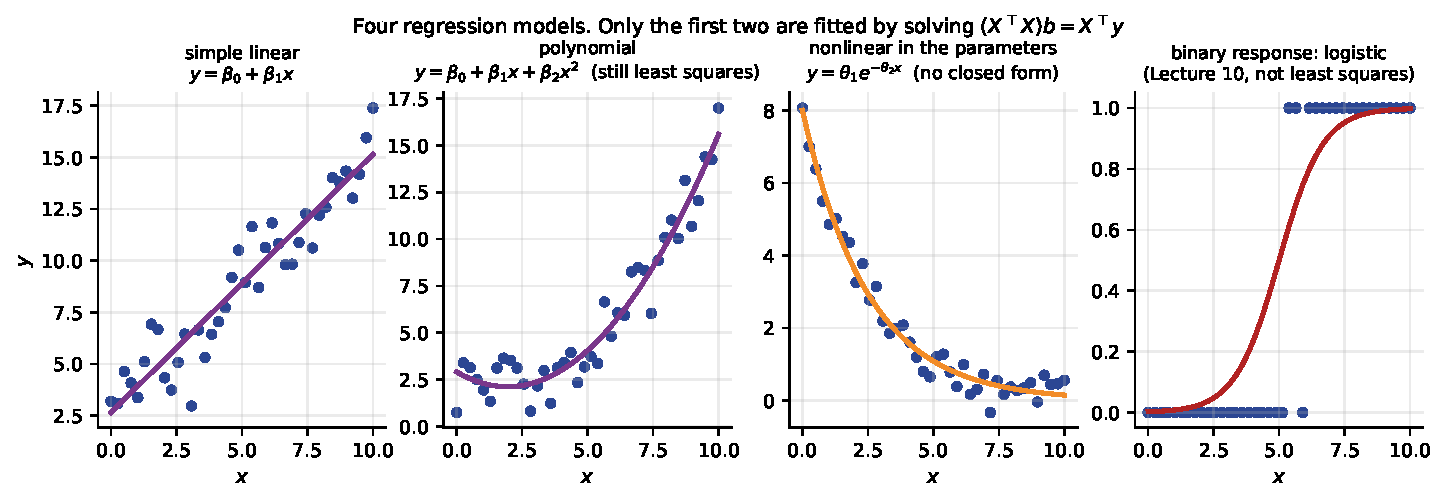
\includegraphics[width=\textwidth]{models.pdf}
  \caption{Four regression models. Panels 1 and 2 are both fitted by solving
    $(X^{\!\top}\!X)b = X^{\!\top}y$; only the columns of $X$ differ. Panel 3
    has a parameter inside an exponential, so no closed form exists. Panel 4
    has a $0/1$ response, so squared error is the wrong objective
    altogether --- that is Lecture 10.}
  \label{fig:models}
\end{figure}

\begin{tryit}[One solver, three models]
Fit degree $1$, $2$ and $3$ polynomials to the same $40$ points, each time by
building a design matrix and solving the normal equations directly.
\begin{lstlisting}
xp = np.linspace(-3.0, 3.0, 40)
rng = np.random.default_rng(0)                  # the one seed for this lecture
yp = 2.0 - 0.5*xp + 0.8*xp**2 + rng.normal(0, 1, 40)
for deg in (1, 2, 3):
    P = np.column_stack([xp**k for k in range(deg + 1)])
    bhat = np.linalg.solve(P.T @ P, P.T @ yp)
    res = yp - P @ bhat
    print(deg, P.shape, np.round(bhat, 4), np.sum(res**2))
\end{lstlisting}
\begin{codeout}
degree 1  design (40, 2)  coefficients [ 4.4626 -0.4485]                  SSE 265.953
degree 2  design (40, 3)  coefficients [ 1.7027 -0.4485  0.8751]          SSE  22.655
degree 3  design (40, 4)  coefficients [ 1.7027 -0.4331  0.8751 -0.0027]  SSE  22.649
\end{codeout}
The data came from $y = 2 - 0.5x + 0.8x^2 + \varepsilon$, and the degree-2 fit
recovers those coefficients to within the noise. \textbf{The same three lines
of code fitted all three models.} Everything this lecture proves about the
straight line transfers unchanged to any design matrix.
\end{tryit}

% =========================================================================
\section{The steps in a regression analysis}
\label{sec:steps}

A regression analysis is a workflow, not a function call. The version below
follows Chatterjee and Hadi's classical presentation and is the one you should
be able to reproduce from memory.

\begin{enumerate}[leftmargin=*]
  \item \textbf{Statement of the problem.} What question are you answering, in
    words, before any data is touched? ``Does body mass index predict disease
    progression?'' is a question. ``Run a regression on the diabetes data'' is
    not.
  \item \textbf{Selection of the variables.} Which quantity is $y$? Which
    quantities could be $x$? In what units, on what scale, measured how?
  \item \textbf{Data collection.} How many rows, gathered how, and split how.
    This is where the Unit IV material lives: cleaning, encoding, scaling and
    a train/test split made \emph{before} anything is fitted.
  \item \textbf{Model specification.} Write the equation down explicitly:
    $y = \beta_0 + \beta_1x + \varepsilon$, with the assumptions you are
    making about $\varepsilon$.
  \item \textbf{Choice of fitting method.} Least squares, maximum likelihood,
    penalised least squares, a robust criterion. This lecture is about the
    first; Lecture 9 shows the first two coincide under Normal noise.
  \item \textbf{Fitting the model.} Compute the estimates. On the scale of
    problems in this course this is the fastest step of the eight.
  \item \textbf{Model validation and criticism.} Do the residuals look like
    noise? Is the held-out error close to the training error? Are the
    assumptions of step 4 defensible? If not, go back to step 4 --- not to
    step 6.
  \item \textbf{Using the model.} Predict, or interpret --- and say which.
\end{enumerate}

\begin{caution}[The analysis is usually lost before step 6]
By the time you type \texttt{fit()} every decision that matters has already
been made. A perfect fit to the wrong response answers the wrong question
perfectly, and no amount of cross-validation will tell you so.
\end{caution}

\subsection{All eight steps, on real patients}
\label{sec:workflow}

\begin{lstlisting}
j = list(dia.feature_names).index("bmi")
xr = Xd[:, j].reshape(-1, 1)
xtr, xte, ytr, yte = train_test_split(xr, yd, test_size=0.25, random_state=0)
m = LinearRegression().fit(xtr, ytr)
\end{lstlisting}
\begin{codeout}
1 problem   : does body mass index predict disease progression?
2 variables : y = progression score; x = bmi (centred and scaled here)
3 data      : 442 patients, 331 train / 111 test
4 model     : y = b0 + b1 x + e
5 method    : least squares
6 fit       : LinearRegression  b0 = 153.2257  b1 = 1016.9235
              by hand           b0 = 153.2257  b1 = 1016.9235
7 check     : train RMSE 61.711   test RMSE 64.664
              training residuals sum to 2.274e-12
              5-fold RMSE 62.605 +/- 2.888
              always predicting ybar gives RMSE 77.006
8 use       : one sd more bmi predicts 49.4 more progression points
\end{codeout}

Three things in that output are worth reading twice. First, line 6: the
library and the hand formula of Section~\ref{sec:derive} agree to four
decimal places, which is the whole point of this lecture. Second, line 7: the
cross-validated RMSE of $62.6$ against $77.0$ for the null model that always
predicts $\bar y$ --- \emph{one} column of \emph{one} measurement removes
about a fifth of the error. Third, also line 7: the test RMSE ($64.7$) is
close to the training RMSE ($61.7$), so there is no over-fitting here. With
two parameters and $331$ rows there was never going to be.

\begin{figure}[htbp]
  \centering
  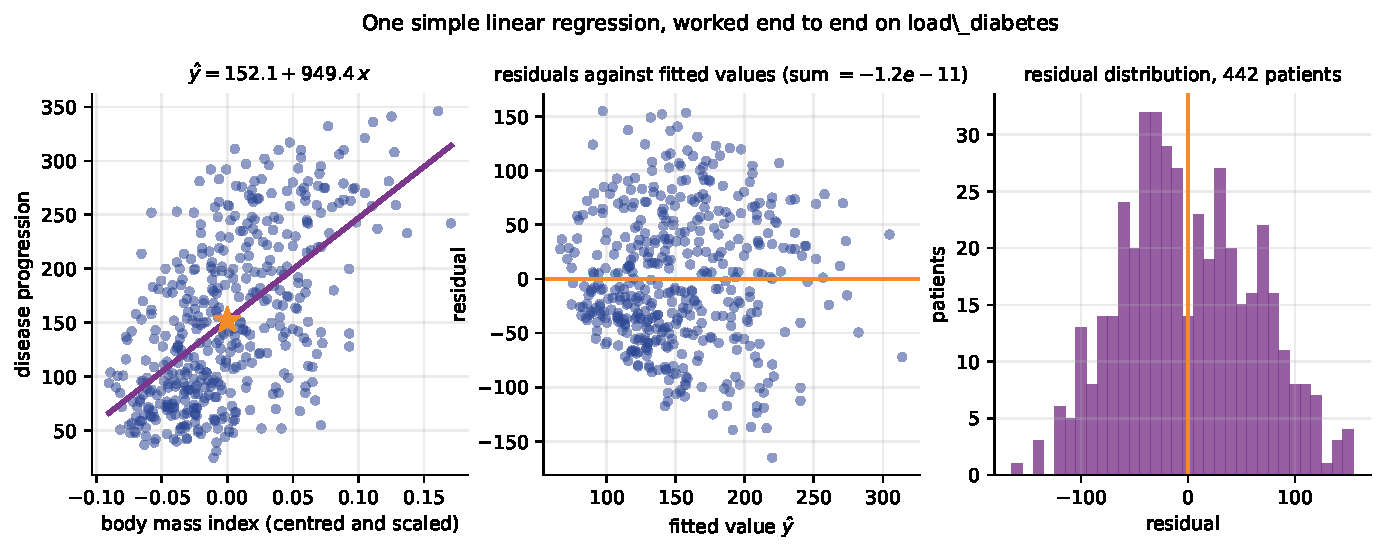
\includegraphics[width=\textwidth]{diabetes.pdf}
  \caption{Step 7 on the fit of Section~\ref{sec:workflow}. Left: the fitted
    line passes through the orange star at $(\bar x,\bar y)$ --- proved in
    Section~\ref{sec:props}. Middle: residuals against fitted values, summing
    to $10^{-11}$ --- also proved there. Right: their distribution. Note that
    the spread widens towards the right of the middle panel, which is a real
    defect of this model and exactly what Lecture 9's diagnostics exist to
    catch.}
  \label{fig:diabetes}
\end{figure}

% =========================================================================
\section{The simple linear regression model}
\label{sec:slr}

\subsection{The model and its assumptions}

\begin{equation}
  y_i \;=\; \beta_0 + \beta_1 x_i + \varepsilon_i, \qquad i = 1,\dots,n .
  \label{eq:slr}
\end{equation}

The four standard assumptions are:

\begin{enumerate}[leftmargin=*]
  \item \textbf{Linearity.} $\mathbb{E}[y \mid x] = \beta_0 + \beta_1 x$: the
    conditional mean of the response really is a straight line in $x$.
  \item \textbf{Independence.} The $\varepsilon_i$ are independent of one
    another. Time series and repeated measures violate this routinely.
  \item \textbf{Constant variance} (homoscedasticity).
    $\mathrm{Var}(\varepsilon_i) = \sigma^2$, the same at every $x$.
  \item \textbf{Zero mean.} $\mathbb{E}[\varepsilon_i] = 0$, so the errors do
    not systematically push the response one way.
\end{enumerate}

Notice what is \emph{not} on the list: Normality. You do not need Normal
errors to compute the least-squares estimates or to establish any property in
Section~\ref{sec:props}. Normality enters in Lecture 9, when we want
confidence intervals, $p$-values and the maximum-likelihood interpretation.

\begin{caution}[Greek letters and Roman letters are different things]
$\beta_0,\beta_1$ describe the population. They are fixed, unknown, and you
will never see them. $b_0,b_1$ are computed from your $n$ rows; collect the
data again and they change. Likewise $\varepsilon_i$ is the unobservable
error and $e_i = y_i - \hat y_i$ is the observable residual. Writing
``$\varepsilon_i = 0.6$'' in an answer script costs marks and, more
importantly, means you have not seen the distinction.
\end{caution}

\subsection{Which line? Choosing a criterion}
\label{sec:criterion}

Infinitely many straight lines pass near a cloud of points. To pick one we
need a criterion: a number, computable from the data and the candidate line,
that we then make as small as possible. Four candidates:

\begin{itemize}[leftmargin=*]
  \item $\sum_i e_i$. \textbf{Useless.} Positive and negative errors cancel,
    so infinitely many lines score exactly zero --- including some very bad
    ones. We will meet three of them in Section~\ref{sec:candidates}.
  \item $\sum_i |e_i|$ (least absolute deviations). Sensible and robust to
    outliers, and it has \emph{no closed form}: $|e|$ has a corner at $e=0$,
    so ``differentiate and set to zero'' is not available. Its minimiser need
    not even be unique.
  \item $\max_i |e_i|$ (minimax, Chebyshev). Lets a single bad row dictate the
    whole line.
  \item $\sum_i e_i^2$ (\textbf{least squares}). Differentiable everywhere,
    convex, and --- the decisive property --- its derivative is
    \emph{linear} in $b_0$ and $b_1$.
\end{itemize}

\begin{keyidea}
Least squares is not chosen because squared error is the truest measure of
wrongness. It is chosen because the derivative of a square is linear, so
setting the gradient to zero produces a \emph{linear system}, which has a
formula. Every other criterion on the list needs a numerical search.
\end{keyidea}

The cost of that convenience is sensitivity: squaring an error of $4$ gives
$16$, so a single distant point dominates the criterion. We measure exactly
how much in Section~\ref{sec:leverage}.

\begin{figure}[htbp]
  \centering
  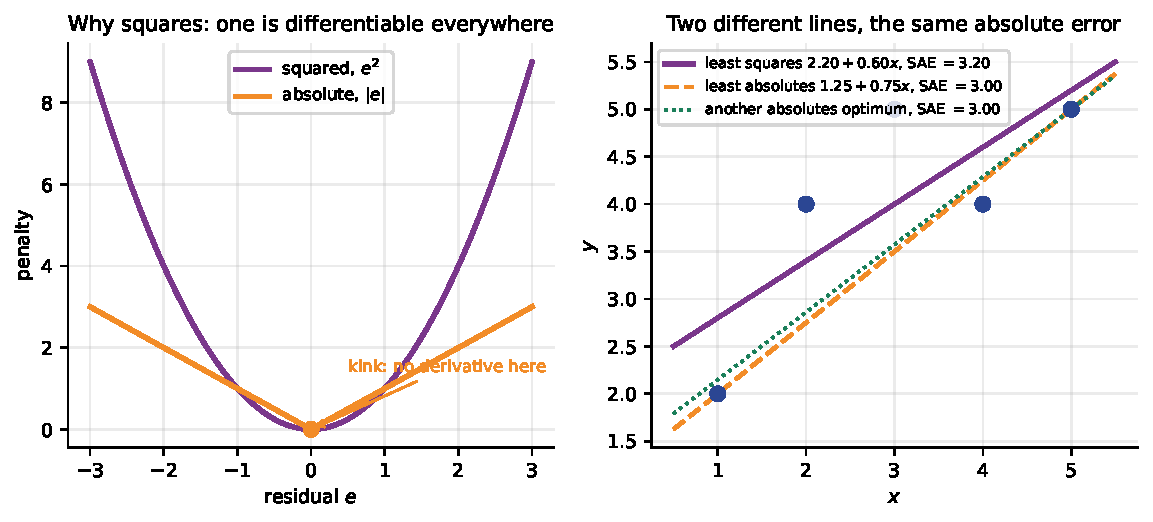
\includegraphics[width=0.92\textwidth]{lossshape.pdf}
  \caption{Left: $|e|$ has a corner at the origin, where it has no derivative;
    $e^2$ is smooth everywhere. Right: on the five points of
    Section~\ref{sec:hand} two different lines achieve \emph{exactly} the same
    total absolute error of $3.00$, so the least-absolute-deviation answer is
    not unique. Least squares always has exactly one answer.}
  \label{fig:lossshape}
\end{figure}

\begin{tryit}[Squares against absolutes on five points]
\begin{codeout}
least squares            b0 = 2.2000  b1 = 0.6000  SSE = 2.4000  SAE = 3.2000
least absolute deviation b0 = 1.2500  b1 = 0.7500  SSE = 3.8750  SAE = 3.0000
the LAD line passes exactly through points 1 and 5
LAD residuals: [ 0.    1.25  1.5  -0.25  0.  ]
a DIFFERENT line   b0 = 1.4340  b1 = 0.7132  SAE = 3.0000
\end{codeout}
Each criterion wins on its own scale, as it must: least squares has the
smaller SSE, least absolute deviations the smaller SAE. The last line is the
point of the box --- \textbf{two different lines, the same absolute error}.
\end{tryit}

% =========================================================================
\section{Least-squares estimation: the derivation}
\label{sec:derive}

This section is the examinable core of the lecture. Work through it with a
pen.

\subsection{The object being minimised}

For a candidate line $\hat y = b_0 + b_1x$ the residual at row $i$ is
$e_i = y_i - b_0 - b_1x_i$, and the criterion is the \textbf{sum of squared
errors}
\begin{equation}
  \mathrm{SSE}(b_0, b_1) \;=\; \sum_{i=1}^{n}\bigl(y_i - b_0 - b_1x_i\bigr)^2 .
  \label{eq:sse}
\end{equation}

Two observations before differentiating, both of which students skip and then
regret.

\begin{enumerate}[leftmargin=*]
  \item In \eqref{eq:sse} the $x_i$ and $y_i$ are \textbf{known numbers}. The
    variables are $b_0$ and $b_1$ --- two of them, whatever $n$ is. SSE is a
    function of two real variables and nothing else.
  \item Every term is a square, so $\mathrm{SSE}\ge 0$ and the surface is a
    bowl. It is bounded below and, as we will confirm in
    Section~\ref{sec:soc}, strictly convex. It therefore has exactly one
    lowest point.
\end{enumerate}

\begin{keyidea}[This is the Lecture 3 objective]
Lecture 3 minimised $J(w) = \frac1n\lVert Xw - y\rVert^2$, which is precisely
$\frac1n\mathrm{SSE}$. Dividing a function by a positive constant does not
move its minimiser. \textbf{Same function, same answer --- and this lecture
finds the answer without stepping.}
\end{keyidea}

\subsection{First-order conditions}

At a minimum both partial derivatives vanish. Differentiate \eqref{eq:sse}
term by term, using the chain rule on $(y_i - b_0 - b_1x_i)^2$. The inner
derivative with respect to $b_0$ is $-1$, and with respect to $b_1$ is
$-x_i$:
\begin{align}
  \frac{\partial\,\mathrm{SSE}}{\partial b_0}
    &= \sum_{i=1}^{n} 2\bigl(y_i - b_0 - b_1x_i\bigr)\cdot(-1)
     = -2\sum_{i=1}^{n}\bigl(y_i - b_0 - b_1x_i\bigr),
       \label{eq:d0}\\
  \frac{\partial\,\mathrm{SSE}}{\partial b_1}
    &= \sum_{i=1}^{n} 2\bigl(y_i - b_0 - b_1x_i\bigr)\cdot(-x_i)
     = -2\sum_{i=1}^{n} x_i\bigl(y_i - b_0 - b_1x_i\bigr).
       \label{eq:d1}
\end{align}

The bracket in both is the residual $e_i$. So the two derivatives are
$-2\sum_i e_i$ and $-2\sum_i x_ie_i$ --- remember that, because setting them
to zero is going to hand us two properties of the fitted line for nothing
(Section~\ref{sec:props}).

\subsection{The normal equations}

Set \eqref{eq:d0} and \eqref{eq:d1} to zero and divide through by $-2$:
\begin{align}
  \sum_i y_i - nb_0 - b_1\sum_i x_i &= 0
    &&\Longrightarrow&
    n\,b_0 + b_1\sum_i x_i &= \sum_i y_i, \label{eq:ne1}\\
  \sum_i x_iy_i - b_0\sum_i x_i - b_1\sum_i x_i^2 &= 0
    &&\Longrightarrow&
    b_0\sum_i x_i + b_1\sum_i x_i^2 &= \sum_i x_iy_i. \label{eq:ne2}
\end{align}
(The middle step uses $\sum_i b_0 = nb_0$, since $b_0$ does not depend on
$i$.)

Equations \eqref{eq:ne1} and \eqref{eq:ne2} are the \textbf{normal
equations}. Look at what has happened: a minimisation over a continuum of
lines has turned into \emph{two linear equations in two unknowns}, whose
coefficients --- $n$, $\sum x_i$, $\sum x_i^2$, $\sum y_i$, $\sum x_iy_i$ ---
are five numbers you can accumulate in a single pass over the data.

\subsection{Solving them}

Divide \eqref{eq:ne1} by $n$ and use $\frac1n\sum_i x_i = \bar x$,
$\frac1n\sum_i y_i = \bar y$:
\begin{equation}
  b_0 + b_1\bar x = \bar y
  \qquad\Longrightarrow\qquad
  b_0 = \bar y - b_1\bar x .
  \label{eq:b0}
\end{equation}
Substitute \eqref{eq:b0} into \eqref{eq:ne2}:
\[
  (\bar y - b_1\bar x)\sum_i x_i + b_1\sum_i x_i^2 = \sum_i x_iy_i ,
\]
and collect the $b_1$ terms on one side:
\[
  b_1\Bigl(\sum_i x_i^2 - \bar x\sum_i x_i\Bigr)
    = \sum_i x_iy_i - \bar y\sum_i x_i .
\]
Now use $\sum_i x_i = n\bar x$ on both sides:
\begin{equation}
  b_1\Bigl(\sum_i x_i^2 - n\bar x^2\Bigr)
    = \sum_i x_iy_i - n\bar x\bar y .
  \label{eq:almost}
\end{equation}

The two brackets in \eqref{eq:almost} have names. Define
\begin{equation}
  S_{xx} = \sum_i (x_i - \bar x)^2, \qquad
  S_{xy} = \sum_i (x_i - \bar x)(y_i - \bar y), \qquad
  S_{yy} = \sum_i (y_i - \bar y)^2 .
  \label{eq:sdefs}
\end{equation}
The identification is a two-line expansion, and it is worth doing once because
it recurs in every regression proof you will meet:
\begin{align*}
  \sum_i (x_i-\bar x)^2
    &= \sum_i x_i^2 - 2\bar x\sum_i x_i + \sum_i \bar x^2
     = \sum_i x_i^2 - 2n\bar x^2 + n\bar x^2
     = \sum_i x_i^2 - n\bar x^2,\\
  \sum_i (x_i-\bar x)(y_i-\bar y)
    &= \sum_i x_iy_i - \bar y\sum_i x_i - \bar x\sum_i y_i + n\bar x\bar y\\
    &= \sum_i x_iy_i - n\bar x\bar y - n\bar x\bar y + n\bar x\bar y
     = \sum_i x_iy_i - n\bar x\bar y .
\end{align*}

So \eqref{eq:almost} reads $b_1S_{xx} = S_{xy}$, and provided $S_{xx}\neq 0$:

\begin{keyidea}[The least-squares estimator]
\[
  \boxed{\;b_1 = \frac{S_{xy}}{S_{xx}}
    = \frac{\sum_i (x_i-\bar x)(y_i-\bar y)}{\sum_i (x_i-\bar x)^2},
  \qquad
  b_0 = \bar y - b_1\bar x .\;}
\]
\end{keyidea}

Two remarks. First, the pair of forms in \eqref{eq:sdefs} --- deviations on
the left, raw sums on the right --- are numerically different: the deviation
form is more accurate, the raw-sum form is what you use in an examination
because $\sum x_i$, $\sum x_i^2$ and $\sum x_iy_i$ come straight off a
five-row table. Second, dividing $S_{xy}$ and $S_{xx}$ by $n-1$ turns them
into the sample covariance and variance, so
\begin{equation}
  b_1 = \frac{\mathrm{cov}(x,y)}{\mathrm{var}(x)}
      = r_{xy}\,\frac{s_y}{s_x},
  \label{eq:slopecorr}
\end{equation}
where $r_{xy}$ is the Pearson correlation. The slope is the correlation,
rescaled by the ratio of the two standard deviations.

\subsection{Second-order condition: it really is a minimum}
\label{sec:soc}

A vanishing gradient marks a minimum, a maximum or a saddle. Differentiate
\eqref{eq:d0} and \eqref{eq:d1} again:
\[
  \frac{\partial^2\mathrm{SSE}}{\partial b_0^2} = 2n, \qquad
  \frac{\partial^2\mathrm{SSE}}{\partial b_1^2} = 2\sum_i x_i^2, \qquad
  \frac{\partial^2\mathrm{SSE}}{\partial b_0\,\partial b_1} = 2\sum_i x_i .
\]
The Hessian is therefore
\begin{equation}
  H = 2\begin{pmatrix} n & \sum_i x_i\\[2pt]
                       \sum_i x_i & \sum_i x_i^2\end{pmatrix},
  \qquad
  \det H = 4\Bigl(n\sum_i x_i^2 - \bigl(\textstyle\sum_i x_i\bigr)^2\Bigr).
  \label{eq:hess}
\end{equation}
Now $n\sum_i x_i^2 - (\sum_i x_i)^2 = n\sum_i x_i^2 - n^2\bar x^2
= n\bigl(\sum_i x_i^2 - n\bar x^2\bigr) = n\,S_{xx}$, so
\begin{equation}
  \det H = 4n\,S_{xx} .
  \label{eq:dethess}
\end{equation}

$H$ is a symmetric $2\times2$ matrix. It is positive definite exactly when its
leading entry and its determinant are both positive. The leading entry is
$2n>0$; the determinant is $4nS_{xx}>0$ whenever the $x_i$ are not all equal.
So:

\begin{keyidea}[Second-order condition]
$H$ is positive definite, SSE is \textbf{strictly convex}, and the stationary
point found above is the \textbf{unique global minimum}. There is one
least-squares line and no other.
\end{keyidea}

The exception is instructive. If every $x_i$ takes the same value then
$S_{xx}=0$, the data is a vertical strip, and no line through it is
determined --- infinitely many lines give the same SSE. The algebra tells you
so by refusing to divide.

\begin{tryit}[The second-order condition, numerically]
\begin{lstlisting}
Xm = np.column_stack([np.ones(n), x])
H  = 2.0 * Xm.T @ Xm                       # Hessian of SSE(b0, b1)
print(H, np.linalg.det(H), np.linalg.eigvalsh(H))
\end{lstlisting}
\begin{codeout}
Hessian of SSE =
 [[ 10.  30.]
 [ 30. 110.]]
d2SSE/db0^2 = 2n      = 10.0
determinant           = 200.0
and 4*n*Sxx           = 200.0
eigenvalues           = [  1.6905 118.3095]
positive definite -> the stationary point is a strict minimum: True
if every x is identical: Sxx = 0.0 and det(X'X) = 0.0 -> no unique fit
\end{codeout}
$\det H = 200$ and $4nS_{xx} = 4\cdot 5\cdot 10 = 200$, exactly as
\eqref{eq:dethess} says. Both eigenvalues are positive, so the bowl curves
upward in every direction.
\end{tryit}

% =========================================================================
\section{The matrix form}
\label{sec:matrix}

Everything above generalises, and the generalisation is shorter than the
special case.

Stack the rows. Let $X$ be the $n\times 2$ \textbf{design matrix} whose first
column is all ones and whose second column is $x$; let $y$ be the $n\times 1$
response and $b = (b_0, b_1)^{\!\top}$. Then $\hat y = Xb$ and
\begin{equation}
  \mathrm{SSE}(b) = \lVert y - Xb\rVert^2 = (y - Xb)^{\!\top}(y - Xb)
    = y^{\!\top}y - 2b^{\!\top}X^{\!\top}y + b^{\!\top}X^{\!\top}Xb .
  \label{eq:matsse}
\end{equation}
(The two cross terms $b^{\!\top}X^{\!\top}y$ and $y^{\!\top}Xb$ are equal
because each is a $1\times1$ matrix and each is the transpose of the other.)
Using $\partial(a^{\!\top}b)/\partial b = a$ and
$\partial(b^{\!\top}Ab)/\partial b = 2Ab$ for symmetric $A$:
\begin{equation}
  \frac{\partial\,\mathrm{SSE}}{\partial b} = -2X^{\!\top}y + 2X^{\!\top}Xb
  \;=\; 0
  \qquad\Longrightarrow\qquad
  \boxed{\;X^{\!\top}\!X\,b = X^{\!\top}y\;}
  \label{eq:matne}
\end{equation}
and, when $X^{\!\top}\!X$ is invertible,
\begin{equation}
  b = (X^{\!\top}\!X)^{-1}X^{\!\top}y .
  \label{eq:ols}
\end{equation}
The Hessian is $2X^{\!\top}\!X$, which is positive definite exactly when $X$
has full column rank --- the general form of the ``not all $x_i$ equal''
condition. Note that \eqref{eq:matne} never mentions the number of columns:
the same three lines fit a multiple regression with fifty predictors, which is
Lecture 11 already done.

\begin{worked}[The matrix route on five points, entirely by hand]
With $x = (1,2,3,4,5)$ and $y = (2,4,5,4,5)$:
\[
  X = \begin{pmatrix}1&1\\1&2\\1&3\\1&4\\1&5\end{pmatrix},\qquad
  X^{\!\top}\!X = \begin{pmatrix} n & \sum x_i\\ \sum x_i & \sum x_i^2
    \end{pmatrix} = \begin{pmatrix}5 & 15\\ 15 & 55\end{pmatrix},\qquad
  X^{\!\top}y = \begin{pmatrix}\sum y_i\\ \sum x_iy_i\end{pmatrix}
    = \begin{pmatrix}20\\ 66\end{pmatrix}.
\]
Here $\sum x_i = 15$, $\sum x_i^2 = 1+4+9+16+25 = 55$, $\sum y_i = 20$ and
$\sum x_iy_i = 2+8+15+16+25 = 66$. Then
\[
  \det(X^{\!\top}\!X) = 5\cdot55 - 15^2 = 275 - 225 = 50 = n\,S_{xx},
  \qquad
  (X^{\!\top}\!X)^{-1} = \frac{1}{50}\begin{pmatrix}55 & -15\\ -15 & 5
    \end{pmatrix},
\]
\[
  b = \frac{1}{50}\begin{pmatrix}55 & -15\\ -15 & 5\end{pmatrix}
      \begin{pmatrix}20\\66\end{pmatrix}
    = \frac{1}{50}\begin{pmatrix}1100 - 990\\ -300 + 330\end{pmatrix}
    = \frac{1}{50}\begin{pmatrix}110\\ 30\end{pmatrix}
    = \begin{pmatrix}2.2\\ 0.6\end{pmatrix}.
\]
The same answer as the scalar formulas, by a completely different route.
\end{worked}

\begin{lstlisting}
Xm  = np.column_stack([np.ones(n), x])
beta = np.linalg.inv(Xm.T @ Xm) @ (Xm.T @ y)
\end{lstlisting}
\begin{codeout}
X'X =
 [[ 5. 15.]
 [15. 55.]]
X'y = [20. 66.]
det(X'X) = 50.0000   and n*Sxx = 50.0000
inv(X'X) =
 [[ 1.1 -0.3]
 [-0.3  0.1]]
beta = inv(X'X) X'y  = [2.2 0.6]
np.linalg.solve      = [2.2 0.6]
np.linalg.lstsq      = [2.2 0.6]
np.linalg.pinv       = [2.2 0.6]
agrees with the scalar formulas to 2.665e-15
\end{codeout}

The printed inverse is the fraction from the board: $55/50 = 1.1$ and
$-15/50 = -0.3$.

\begin{caution}[Never write \texttt{np.linalg.inv} in real code]
It gives the same answer here, and worse answers than
\texttt{np.linalg.solve} or \texttt{np.linalg.lstsq} whenever
$X^{\!\top}\!X$ is close to singular --- which, as Lecture 6 showed with the
dummy variable trap (condition number $1.2\times10^{15}$), is not a rare
event. Use \texttt{solve} when you know the matrix is well conditioned and
\texttt{lstsq} when you do not. \texttt{LinearRegression} uses
\texttt{lstsq} internally.
\end{caution}

% =========================================================================
\section{The five-point calculation, by hand and in code}
\label{sec:hand}

\subsection{By hand}

Five students. $x$ is hours of revision in the week before a quiz; $y$ is the
quiz score out of ten. The numbers are chosen so that every intermediate
quantity is an integer or a clean decimal.

\begin{worked}[Least squares on five points]
\begin{center}\small
\begin{tabular}{@{}lrrrrr|r@{}}
  \toprule
  & & & & & & $\Sigma$\\
  \midrule
  $x$ & $1$ & $2$ & $3$ & $4$ & $5$ & $15$\\
  $y$ & $2$ & $4$ & $5$ & $4$ & $5$ & $20$\\
  \midrule
  $x-\bar x$ & $-2$ & $-1$ & $0$ & $1$ & $2$ & $0$\\
  $y-\bar y$ & $-2$ & $0$ & $1$ & $0$ & $1$ & $0$\\
  $(x-\bar x)^2$ & $4$ & $1$ & $0$ & $1$ & $4$ & $\mathbf{10}$\\
  $(x-\bar x)(y-\bar y)$ & $4$ & $0$ & $0$ & $0$ & $2$ & $\mathbf{6}$\\
  $(y-\bar y)^2$ & $4$ & $0$ & $1$ & $0$ & $1$ & $\mathbf{6}$\\
  \bottomrule
\end{tabular}
\end{center}
\[
  \bar x = \tfrac{15}{5} = 3, \qquad \bar y = \tfrac{20}{5} = 4, \qquad
  S_{xx} = 10, \qquad S_{xy} = 6, \qquad S_{yy} = 6 .
\]
\[
  b_1 = \frac{S_{xy}}{S_{xx}} = \frac{6}{10} = 0.6,
  \qquad
  b_0 = \bar y - b_1\bar x = 4 - 0.6\times 3 = 2.2 .
\]
\[
  \boxed{\hat y = 2.2 + 0.6\,x}
\]
An extra hour of revision is associated with $0.6$ more marks. Check against
the raw-sum forms: $S_{xx} = \sum x_i^2 - n\bar x^2 = 55 - 5(9) = 10$ and
$S_{xy} = \sum x_iy_i - n\bar x\bar y = 66 - 5(3)(4) = 6$. Same numbers.
\end{worked}

\begin{codeout}
n    = 5
xbar = 3.0000   ybar = 4.0000
Sxx  = 10.0000   Sxy  = 6.0000   Syy = 6.0000
b1   = Sxy/Sxx        = 0.6000
b0   = ybar - b1*xbar = 2.2000
fitted line: yhat = 2.2 + 0.6 x
\end{codeout}

\begin{figure}[htbp]
  \centering
  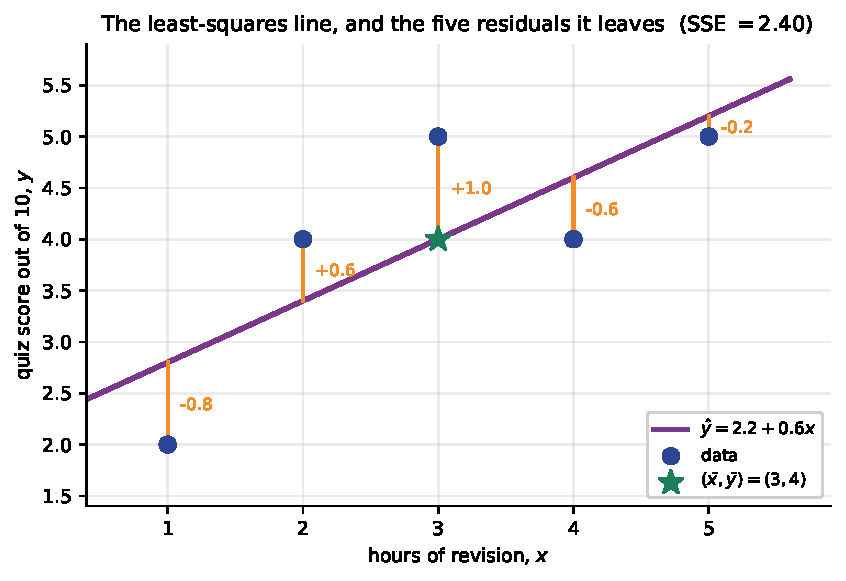
\includegraphics[width=0.72\textwidth]{fitline.pdf}
  \caption{The least-squares line and the five residuals. They sum to exactly
    zero, and the green star at $(\bar x,\bar y) = (3,4)$ lies on the line.
    Both facts are forced by the normal equations, as
    Section~\ref{sec:props} shows.}
  \label{fig:fitline}
\end{figure}

\begin{figure}[htbp]
  \centering
  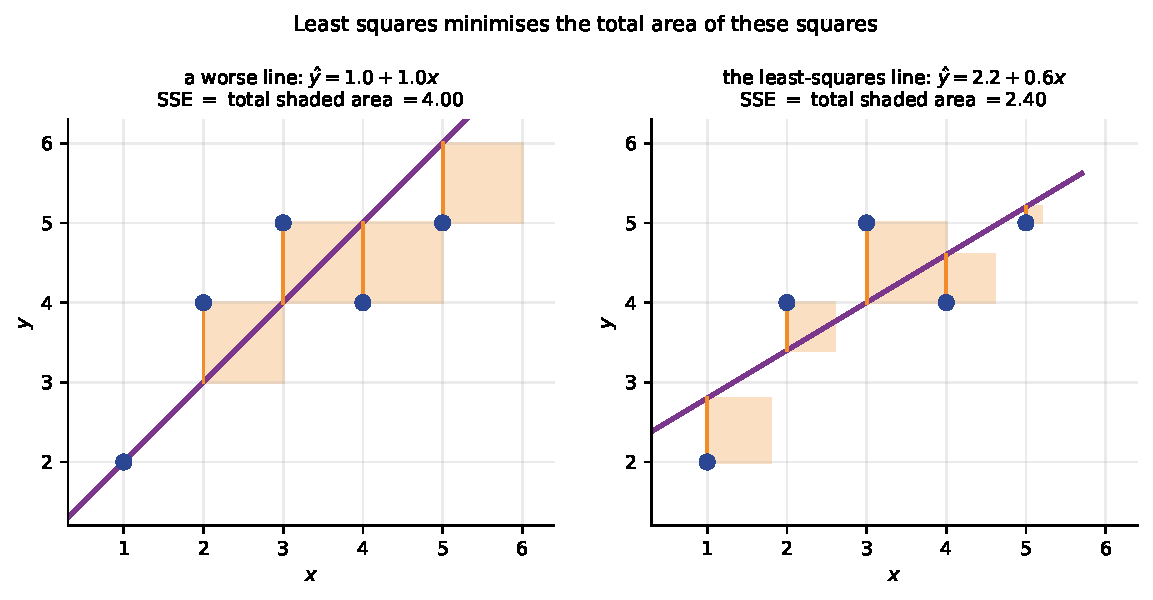
\includegraphics[width=0.9\textwidth]{squares.pdf}
  \caption{Each residual drawn as a literal square of side $|e_i|$. The SSE is
    the total shaded area: $4.00$ for $\hat y = 1.0 + 1.0x$ and $2.40$ for the
    least-squares line. Least squares slides the line until that area is as
    small as it can be.}
  \label{fig:squares}
\end{figure}

\subsection{And in code}

\begin{lstlisting}
x = np.array([1.0, 2.0, 3.0, 4.0, 5.0])
y = np.array([2.0, 4.0, 5.0, 4.0, 5.0])
xbar, ybar = x.mean(), y.mean()
Sxx = np.sum((x - xbar)**2)
Sxy = np.sum((x - xbar) * (y - ybar))
b1  = Sxy / Sxx
b0  = ybar - b1 * xbar

p  = np.polyfit(x, y, 1)                       # returns [slope, intercept]
lr = LinearRegression().fit(x.reshape(-1, 1), y)
\end{lstlisting}
\begin{codeout}
by hand          b0 = 2.200000000000   b1 = 0.600000000000
np.polyfit       b0 = 2.200000000000   b1 = 0.600000000000
LinearRegression b0 = 2.200000000000   b1 = 0.600000000000
max abs difference, hand vs polyfit          4.441e-16
max abs difference, hand vs LinearRegression 0.000e+00
\end{codeout}

Not ``close'': \texttt{LinearRegression} matched the hand arithmetic
\textbf{exactly}, and \texttt{np.polyfit} differs by one unit in the last
place of a double because it routes through a singular value decomposition.

\begin{keyidea}
The library is not doing anything you did not just do on paper. It is doing it
faster, and with better numerics on problems where $X^{\!\top}\!X$ is
ill-conditioned. If you can compute $b_1 = S_{xy}/S_{xx}$ by hand, you know
what \texttt{fit()} does.
\end{keyidea}

\subsection{Four candidate lines}
\label{sec:candidates}

Before accepting the formula, check that the line it produces really is the
best of the alternatives, and check something subtler at the same time.

\begin{center}\small
\begin{tabular}{@{}lrrr@{}}
  \toprule
  Candidate & SSE & $\sum_i e_i$ & $\sum_i x_ie_i$\\
  \midrule
  A: $\hat y = 2.0 + 0.7x$ & $2.5500$ & $-0.5000$ & $-2.5000$\\
  B: $\hat y = 2.2 + 0.6x$ & $\mathbf{2.4000}$ & $\mathbf{0.0000}$ &
    $\mathbf{0.0000}$\\
  C: $\hat y = 2.5 + 0.5x$ & $2.5000$ & $0.0000$ & $+1.0000$\\
  D: $\hat y = 1.0 + 1.0x$ & $4.0000$ & $0.0000$ & $-4.0000$\\
  \bottomrule
\end{tabular}
\end{center}

\begin{caution}[$\sum e_i = 0$ is necessary, not sufficient]
Three of the four lines have residuals summing to zero, and two of those three
are worse than the least-squares line. Zero residual sum is only
\emph{one} of the two normal equations. B is the only candidate that also
satisfies $\sum_i x_ie_i = 0$, and B is the one with the smallest SSE. A
student who checks only the first condition has checked half the answer.
\end{caution}

\begin{figure}[htbp]
  \centering
  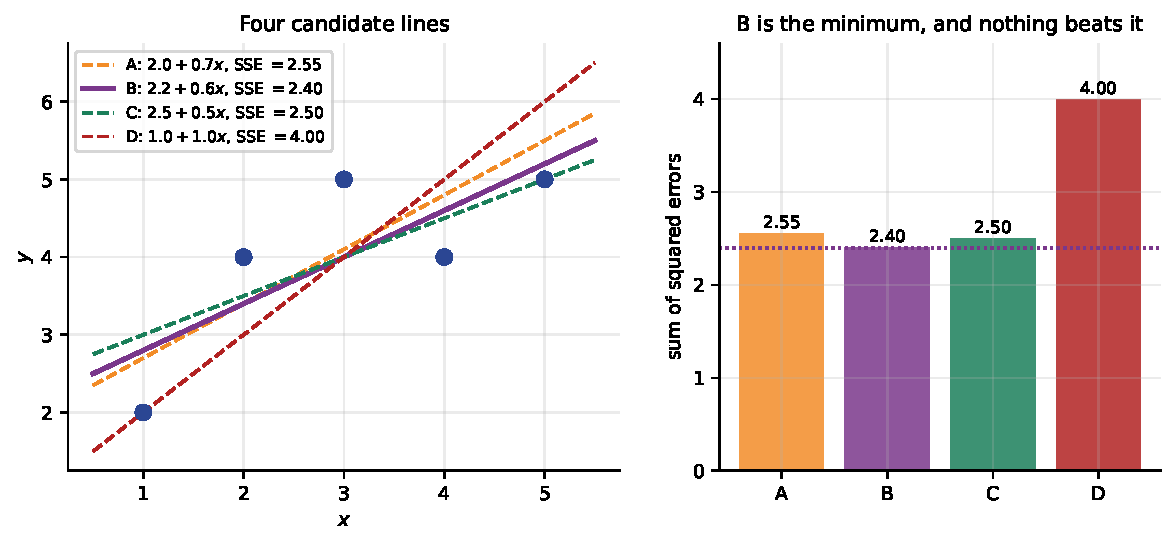
\includegraphics[width=0.94\textwidth]{candidates.pdf}
  \caption{The four candidates and their scores. C looks almost as good as B
    and scores $2.50$ against $2.40$: near the bottom of a bowl the surface is
    flat, which is also why gradient descent takes so long to finish
    (Section~\ref{sec:gd}).}
  \label{fig:candidates}
\end{figure}

% =========================================================================
\section{The line of best fit and its properties}
\label{sec:props}

Four properties follow immediately from the two normal equations. They are
short proofs and they are examined.

\subsection{Property 1: the residuals sum to zero}

Equation \eqref{eq:ne1} was $\sum_i(y_i - b_0 - b_1x_i) = 0$, and the bracket
is $e_i$. Hence
\begin{equation}
  \sum_{i=1}^{n} e_i = 0,
  \qquad\text{and dividing by } n, \qquad
  \bar{\hat y} = \bar y .
  \label{eq:sumzero}
\end{equation}
The fitted values have the same mean as the observations.

\begin{caution}[Only with an intercept]
Equation \eqref{eq:sumzero} \emph{is} the $\partial\mathrm{SSE}/\partial b_0 =
0$ condition. Remove the intercept from the model and there is no such
equation, and no such guarantee. See Section~\ref{sec:nointercept}, where the
residuals of a no-intercept fit sum to $+2$.
\end{caution}

\subsection{Property 2: the line passes through the centroid}

From \eqref{eq:b0}, $b_0 = \bar y - b_1\bar x$, so evaluating the fitted line
at $x=\bar x$:
\begin{equation}
  \hat y(\bar x) = b_0 + b_1\bar x = (\bar y - b_1\bar x) + b_1\bar x
    = \bar y .
  \label{eq:centroid}
\end{equation}
Every least-squares line with an intercept passes through
$(\bar x, \bar y)$. This is a good sanity check on any hand computation: if
your line misses the centroid, you have made an arithmetic error.

\subsection{Property 3: residuals are orthogonal to the predictor}

Equation \eqref{eq:ne2} says $\sum_i x_i(y_i - b_0 - b_1x_i) = 0$, that is
\begin{equation}
  \sum_{i=1}^{n} x_ie_i = 0 .
  \label{eq:orthx}
\end{equation}
Combining with \eqref{eq:sumzero},
\begin{equation}
  \sum_i \hat y_ie_i = \sum_i (b_0 + b_1x_i)e_i
    = b_0\underbrace{\sum_i e_i}_{0} + b_1\underbrace{\sum_i x_ie_i}_{0}
    = 0 .
  \label{eq:orthyhat}
\end{equation}
Geometrically the residual vector is orthogonal both to the column of ones and
to the column $x$, hence to every vector in the plane they span --- which is
to say, \textbf{there is no linear signal left in the residuals}. If you
regressed $e$ on $x$ you would get a slope of exactly zero.

\subsection{Property 4: the sum of squares decomposes}

Write $y_i - \bar y = (\hat y_i - \bar y) + e_i$ and square:
\[
  \sum_i (y_i-\bar y)^2 = \sum_i(\hat y_i - \bar y)^2 + \sum_i e_i^2
    + 2\sum_i (\hat y_i - \bar y)e_i .
\]
The cross term is $2\sum_i \hat y_ie_i - 2\bar y\sum_i e_i = 0$ by
\eqref{eq:orthyhat} and \eqref{eq:sumzero}, so
\begin{equation}
  \underbrace{\sum_i (y_i - \bar y)^2}_{\mathrm{SST}}
    = \underbrace{\sum_i (\hat y_i - \bar y)^2}_{\mathrm{SSR}}
    + \underbrace{\sum_i e_i^2}_{\mathrm{SSE}} .
  \label{eq:anova}
\end{equation}
Total variation splits into the part the line explains and the part it does
not. One further identity, obtained by substituting
$\hat y_i - \bar y = b_1(x_i - \bar x)$:
\begin{equation}
  \mathrm{SSR} = b_1^2 S_{xx} = \frac{S_{xy}^2}{S_{xx}} .
  \label{eq:ssr}
\end{equation}

\subsection{All four, on the five points}

\begin{codeout}
  x      y     yhat   residual
  1    2.0    2.80     -0.80
  2    4.0    3.40      0.60
  3    5.0    4.00      1.00
  4    4.0    4.60     -0.60
  5    5.0    5.20     -0.20
sum of residuals        -0.000000000000000
sum of x_i * e_i        -0.000000000000000
sum of yhat_i * e_i     -0.000000000000001
mean of yhat = 4.0000   and ybar = 4.0000
the line at xbar = 3.0 gives 4.0000   and ybar = 4.0000
\end{codeout}
\begin{codeout}
SSE (residual)  = 2.4000
SSR (explained) = 3.6000
SST (total)     = 6.0000
SSR + SSE       = 6.0000   and SST = 6.0000
check: SSR = Sxy^2/Sxx = 3.6000
mean squared error of the fit = SSE/n = 0.4800
correlation r = Sxy/sqrt(Sxx*Syy) = 0.7746
and b1 = r * sd(y)/sd(x) = 0.7746 * 1.2247/1.5811 = 0.6000
r^2 = 0.6000, and SSR/SST = 0.6000 -- the same number (Lecture 9 names it)
\end{codeout}

$\mathrm{SSR} = S_{xy}^2/S_{xx} = 36/10 = 3.6$ exactly as \eqref{eq:ssr}
predicts, and \eqref{eq:slopecorr} reproduces the slope from the correlation.
The last line is a forward reference: $\mathrm{SSR}/\mathrm{SST} = 0.6$ and
$r^2 = 0.6$ are the same number, and Lecture 9 gives it a name and a warning.

\subsection{Drop the intercept and watch Property 1 die}
\label{sec:nointercept}

Fit $\hat y = b_1x$ instead. There is now one parameter, hence one normal
equation --- the one from $\partial/\partial b_1$ --- and minimising
$\sum_i(y_i - b_1x_i)^2$ gives $-2\sum_i x_i(y_i - b_1x_i) = 0$, so
$b_1 = \sum_i x_iy_i / \sum_i x_i^2$.

\begin{lstlisting}
b1_noint = np.sum(x * y) / np.sum(x * x)      # fit y = b1 x, no intercept
\end{lstlisting}
\begin{codeout}
no-intercept fit  yhat = 1.2000 x
residuals         [ 0.8  1.6  1.4 -0.8 -1. ]
sum of residuals  +2.0000   (NOT zero)
sum of x_i * e_i  +1.7764e-15   (still zero -- that equation was solved)
SSE               6.8000  against 2.4000 with an intercept
\end{codeout}

The residuals now sum to $+2$, and the SSE nearly trebles. Note what
\emph{did} survive: $\sum x_ie_i$ is still zero, because that equation was the
one we solved.

\begin{keyidea}
``The residuals of a regression sum to zero'' is a statement about the model
containing an intercept, not about least squares. Whenever you see the claim,
the words ``with an intercept'' are doing all the work.
\end{keyidea}

% =========================================================================
\section{How precise is the line? $S_{xx}$ is the answer}
\label{sec:precision}

The estimates $b_0$ and $b_1$ are computed from data, and data is noisy, so
they are random quantities. Under the four assumptions of
Section~\ref{sec:slr} one can show
\begin{equation}
  \mathbb{E}[b_1] = \beta_1, \qquad
  \mathrm{Var}(b_1) = \frac{\sigma^2}{S_{xx}}, \qquad
  \mathrm{Var}(b_0) = \sigma^2\left(\frac1n + \frac{\bar x^2}{S_{xx}}\right).
  \label{eq:varb}
\end{equation}
(The first says least squares is \emph{unbiased}; the Gauss--Markov theorem
strengthens this to ``no other linear unbiased estimator has smaller
variance''. Lecture 9 does the derivations properly.)

Read the middle formula. $S_{xx}$ sits in the denominator, so the more spread
out the $x$ values, the more precisely you learn the slope --- with the same
number of rows, at no extra cost.

\begin{keyidea}[A design lesson worth money]
If you can \emph{choose} where to observe --- a calibration, an experiment, a
load test --- put your observations at the extremes of the usable range rather
than clustering them in the middle. Same $n$, smaller standard error.
\end{keyidea}

\begin{tryit}[Measure it: 4000 refits at four spreads]
\begin{lstlisting}
rng = np.random.default_rng(0)                  # the one seed for this lecture
for spread in (0.5, 1.0, 2.0, 4.0):
    xs = np.linspace(-spread, spread, 20)
    Sxx_s = np.sum((xs - xs.mean())**2)
    slopes = [np.sum((xs - xs.mean())*(ys - ys.mean())) / Sxx_s
              for ys in (1.0 + 2.0*xs + rng.normal(0, 1, 20)
                         for _ in range(4000))]
\end{lstlisting}
\begin{codeout}
half-range of x    Sxx    sd of 4000 fitted slopes   sigma/sqrt(Sxx)
         0.5    1.842                  0.7237            0.7368
         1.0    7.368                  0.3683            0.3684
         2.0   29.474                  0.1859            0.1842
         4.0  117.895                  0.0932            0.0921
\end{codeout}
Eight times the range, $64$ times $S_{xx}$, and $7.8$ times the precision. The
measured column and the theoretical column agree to three decimal places, so
\eqref{eq:varb} is not decoration.
\end{tryit}

\begin{figure}[htbp]
  \centering
  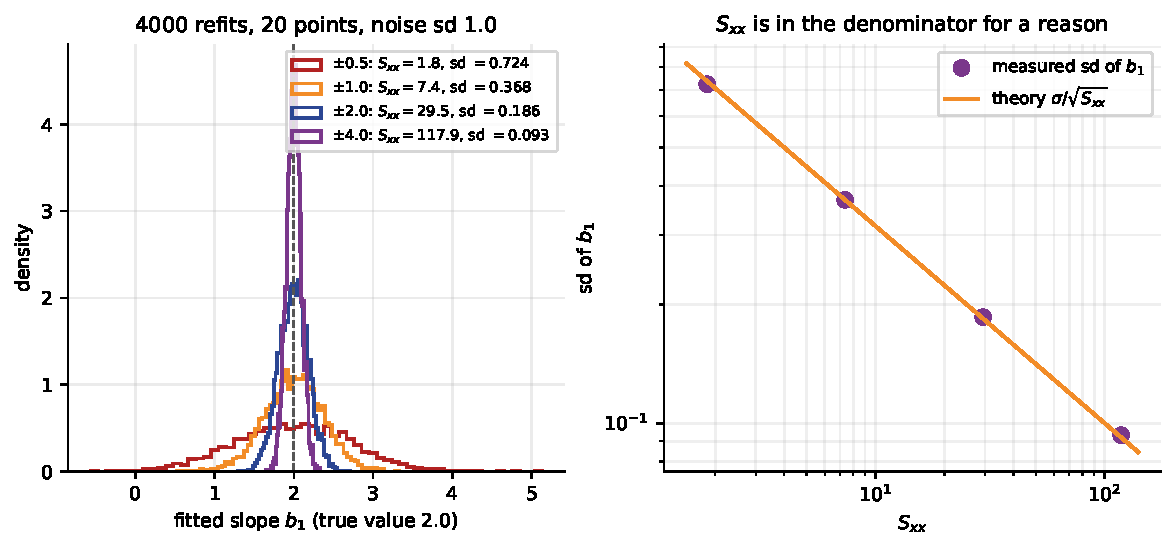
\includegraphics[width=0.94\textwidth]{sxx.pdf}
  \caption{Left: four sampling distributions of $b_1$, all centred on the true
    value $2.0$ --- least squares is unbiased whatever the spread --- with
    very different widths. Right: the measured widths against
    $\sigma/\sqrt{S_{xx}}$ on logarithmic axes.}
  \label{fig:sxx}
\end{figure}

% =========================================================================
\section{Two roads to the same answer}
\label{sec:gd}

\subsection{The connection to Lecture 3}

Lecture 3 minimised, for a linear model,
\[
  J(w) = \frac1n\lVert Xw - y\rVert^2,
  \qquad
  \nabla J(w) = \frac{2}{n}X^{\!\top}(Xw - y),
  \qquad
  w \leftarrow w - \eta\,\nabla J(w),
\]
and iterated until the parameters stopped moving. Compare with
\eqref{eq:matne}: setting that same gradient to zero gives
$X^{\!\top}Xw = X^{\!\top}y$, which is a linear system you solve.

\begin{keyidea}
Gradient descent \emph{approaches} the point where the gradient vanishes.
Least squares \emph{solves} for it. They are not competing methods for
different problems --- for this problem they are two routes to the same point.
Lecture 3 iterated because in general $\nabla J = 0$ cannot be solved in
closed form; for a linear model with squared loss, it can.
\end{keyidea}

\subsection{On the five points}

\begin{lstlisting}
def grad(theta):
    r = y - (theta[0] + theta[1] * x)
    return np.array([-2.0 * r.sum(), -2.0 * np.sum(x * r)])

theta = np.array([0.0, 0.0])
for k in range(1, 4001):
    theta = theta - 0.01 * grad(theta)
\end{lstlisting}
\begin{codeout}
 iter        b0        b1        SSE   max|theta-theta*|
    1    0.4000    1.3200     8.2320        1.80e+00
    2    0.3640    1.0680     5.5234        1.84e+00
    5    0.4655    1.0807     5.1381        1.73e+00
   10    0.6072    1.0412     4.7089        1.59e+00
   50    1.3946    0.8231     2.9903        8.05e-01
  200    2.1376    0.6173     2.4035        6.24e-02
 1000    2.2000    0.6000     2.4000        7.44e-08
 4000    2.2000    0.6000     2.4000        1.24e-14
closed form              2.2000    0.6000     2.4000
gradient descent matched the closed form to 4 decimals at iteration 619
\end{codeout}

Six hundred and nineteen iterations to reproduce one division. And look at the
SSE column: after $200$ steps the loss is $2.4035$ against the optimal
$2.4000$, while the parameters are still $0.06$ away. \textbf{Near the bottom
of a bowl the surface is flat, so a large parameter error costs almost no
loss} --- which is exactly why choosing $\eta$ and a stopping rule felt so
fiddly in Lecture 3.

\begin{figure}[htbp]
  \centering
  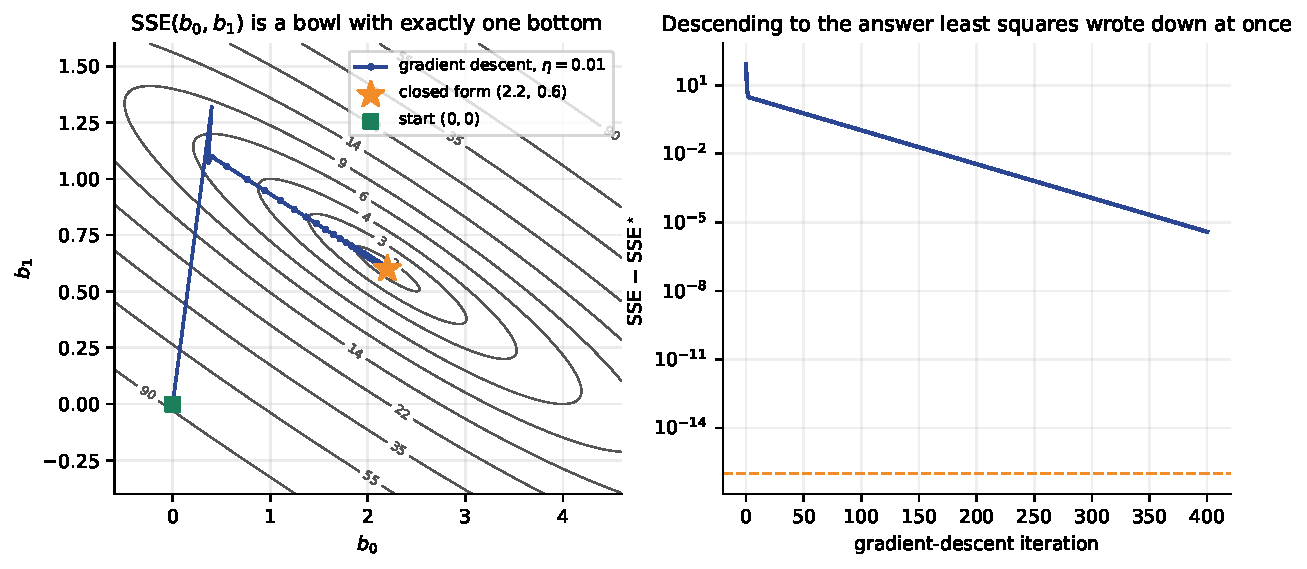
\includegraphics[width=0.94\textwidth]{bowl.pdf}
  \caption{Left: contours of $\mathrm{SSE}(b_0,b_1)$ with the gradient-descent
    path from $(0,0)$ and the closed-form solution as a star. The contours are
    tilted ellipses because $b_0$ and $b_1$ are correlated --- the off-diagonal
    $\sum x_i$ of $X^{\!\top}\!X$ --- so descent zig-zags down a valley, which
    is the Lecture 6 ravine picture again. Right: the gap to the optimal loss
    on a logarithmic scale.}
  \label{fig:bowl}
\end{figure}

\subsection{And on 442 real patients}

The same comparison on \texttt{load\_diabetes}, \texttt{bmi} against
progression. Gradient descent is run on standardised $x$ (Lecture 6's lesson:
otherwise one step size does not work) and the coefficients are then unwound
to the original units.

\begin{lstlisting}
xs = StandardScaler().fit(xb)
Z  = np.column_stack([np.ones(len(yd)), xs.transform(xb).ravel()])
wz = np.zeros(2)
for it in range(2000):
    wz = wz - 0.1 * (2.0 / len(yd)) * (Z.T @ (Z @ wz - yd))
b1_gd = wz[1] / xs.scale_[0]
b0_gd = wz[0] - wz[1] * xs.mean_[0] / xs.scale_[0]

sgd = make_pipeline(StandardScaler(),            # the stochastic route
      SGDRegressor(loss="squared_error", penalty=None,
                   learning_rate="constant", eta0=0.01,
                   max_iter=50000, tol=1e-10,
                   random_state=0))              # the one seed for this lecture
sgd.fit(xb, yd)
\end{lstlisting}
\begin{codeout}
full-batch GD     1 steps   b0 =   30.4267   b1 =  189.8871   J = 20008.2328
full-batch GD    10 steps   b0 =  135.7983   b1 =  847.4904   J = 4180.8086
full-batch GD   100 steps   b0 =  152.1335   b1 =  949.4353   J = 3890.4566
full-batch GD   500 steps   b0 =  152.1335   b1 =  949.4353   J = 3890.4566
full-batch GD  2000 steps   b0 =  152.1335   b1 =  949.4353   J = 3890.4566
closed form               b0 =  152.1335   b1 =  949.4353   J = 3890.4566
difference in the slope   4.547e-13 (relative 4.441e-16)
SGDRegressor (stochastic) b0 =  149.5577   b1 =  891.1257   J = 3904.7835
the stochastic version stops 6.1% away from the slope: that is the
noise floor of Lecture 3, not a bug
\end{codeout}

One hundred steps of full-batch descent reproduce
$(X^{\!\top}\!X)^{-1}X^{\!\top}y$ to fifteen significant figures.
\texttt{SGDRegressor} with a constant step size lands $6.1\%$ away on the
slope, and that is not a defect of the implementation: Lecture 3 established
that a constant-step stochastic method converges to a \emph{region} around the
optimum, not to a point. Report it, do not hide it.

\subsection{So which do you use?}

\begin{center}\small
\begin{tabular}{@{}lll@{}}
  \toprule
  & \textbf{Closed form} & \textbf{Gradient descent}\\
  \midrule
  Cost & $O(nd^2 + d^3)$, one pass & $O(nd)$ per step, many steps\\
  Memory & needs $X^{\!\top}\!X$ or all of $X$ & one mini-batch at a time\\
  Tuning & none & step size, schedule, batch size, stopping\\
  Answer & exact & as close as you can afford\\
  Fails when & $d$ large; $X^{\!\top}\!X$ singular & almost never, slowly\\
  Extends to & squared loss on a linear model & anything differentiable\\
  \bottomrule
\end{tabular}
\end{center}

Rule of thumb: small $d$ (say up to a few thousand columns), data in memory,
squared loss, linear model --- \textbf{use the closed form}, which is what
\texttt{LinearRegression} does. Enormous $n$ or $d$, streaming data, or any
model outside that family --- descend. Logistic regression, two lectures
away, has no closed form at all, which is why Lecture 3 came first.

% =========================================================================
\section{What least squares will not tell you}
\label{sec:limits}

\subsection{Leverage: not all rows are equal}
\label{sec:leverage}

The slope is $b_1 = \sum_i(x_i-\bar x)(y_i-\bar y)/S_{xx}$, so row $i$ enters
weighted by $(x_i - \bar x)$. A row sitting at $x_i = \bar x$ has weight zero
and \emph{cannot} influence the slope, however wrong its $y$ is. The
\textbf{leverage}
\begin{equation}
  h_i = \frac1n + \frac{(x_i - \bar x)^2}{S_{xx}}
  \label{eq:lev}
\end{equation}
measures how much row $i$ can pull the fit; the second term is the part that
concerns the slope.

\begin{codeout}
point moved         b0       b1    change in b1
none                2.2000   0.6000        +0.0000
y at x=3: 5 -> 9    3.0000   0.6000        +0.0000
y at x=5: 5 -> 9    0.6000   1.4000        +0.8000
y at x=1: 2 -> -2  -1.0000   1.4000        +0.8000
leverage (x-xbar)^2/Sxx: [0.4 0.1 0.  0.1 0.4]
\end{codeout}

The same $+4$ error in $y$ leaves the slope completely unchanged when it
happens at $x=\bar x$ and moves it by $+0.8$ --- more than doubling it --- when
it happens at the end of the range. Two of the five rows carry $80\%$ of the
slope leverage between them.

\begin{caution}
``Is this point an outlier?'' is the wrong question. A point far from the
others \emph{in $y$} may do no harm; a point far from the others \emph{in $x$}
can determine the answer on its own. Ask where a suspicious row sits in $x$
before you ask how odd its $y$ is.
\end{caution}

\begin{figure}[htbp]
  \centering
  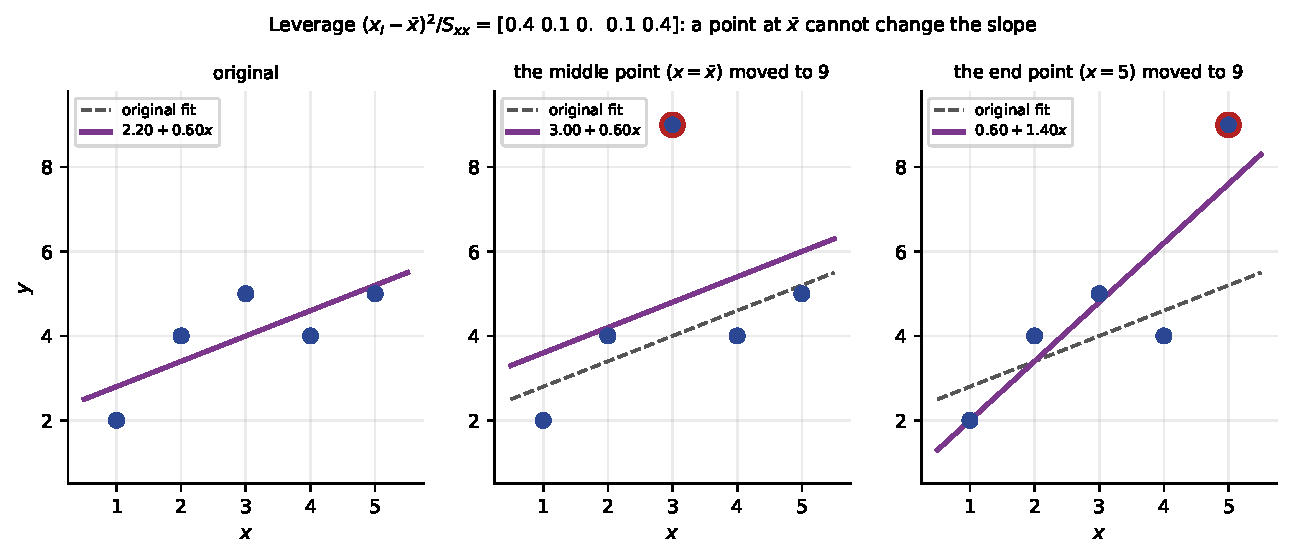
\includegraphics[width=\textwidth]{leverage.pdf}
  \caption{The same $+4$ change in one $y$ value. In the middle panel the line
    lifts and keeps its slope; in the right panel it pivots.}
  \label{fig:leverage}
\end{figure}

\subsection{Anscombe's quartet}
\label{sec:anscombe}

Francis Anscombe constructed four eleven-point datasets in 1973. Every
statistic least squares computes is the same for all four.

\begin{codeout}
set   xbar   ybar     Sxx     Sxy      b0      b1      SSE
I      9.00   7.50   110.00   55.01  3.0001  0.5001  13.7627
II     9.00   7.50   110.00   55.00  3.0009  0.5000  13.7763
III    9.00   7.50   110.00   54.97  3.0025  0.4997  13.7562
IV     9.00   7.50   110.00   54.99  3.0017  0.4999  13.7425
\end{codeout}

\begin{figure}[htbp]
  \centering
  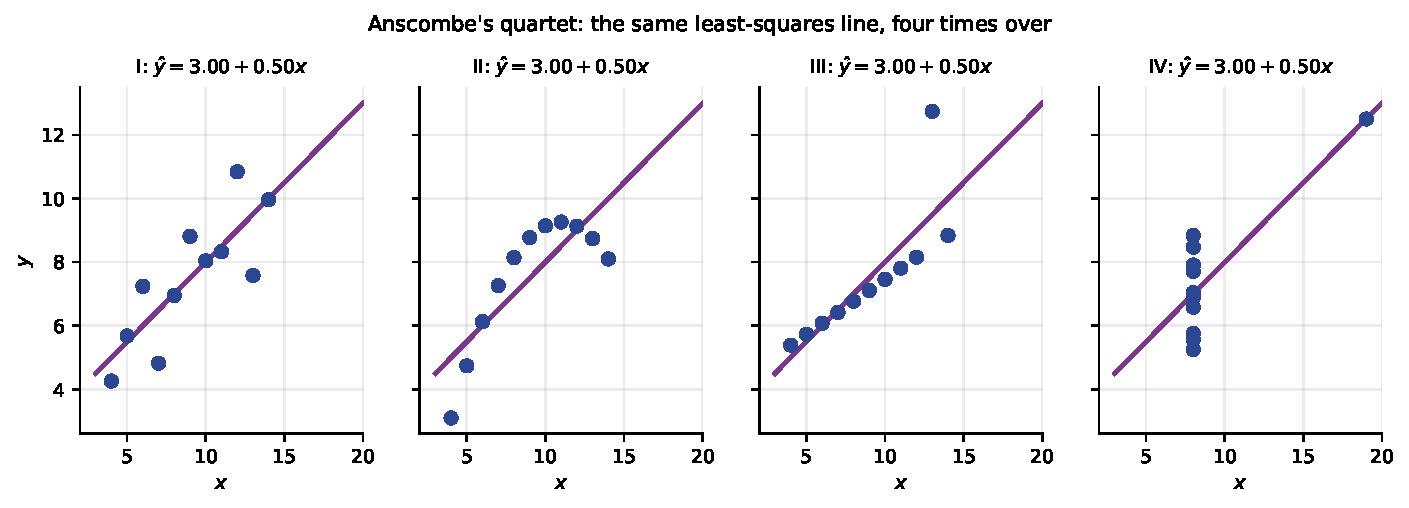
\includegraphics[width=\textwidth]{anscombe.pdf}
  \caption{Anscombe's quartet. Every column of the table above agrees to two
    decimal places; the pictures do not agree at all.}
  \label{fig:anscombe}
\end{figure}

Dataset I is a reasonable linear fit. Dataset II is a \emph{parabola} --- the
model is simply wrong, and no amount of extra data would fix it. Dataset III
is a perfect straight line plus one contaminated point. Dataset IV has ten
observations at $x=8$ and a single observation at $x=19$ whose leverage is
$1.0$: that one point determines the slope, and deleting it leaves $S_{xx}=0$
and no fit at all.

\begin{keyidea}
Least squares always returns a line. Whether the line means anything is a
separate question, and the estimates alone cannot answer it. Plot the data,
and plot the residuals --- which is Lecture 9's business.
\end{keyidea}

\subsection{And it says nothing about causation}

\begin{codeout}
feature        b1        b0        SSE      corr(x,y)
bmi         949.435   152.133   1719581.8      0.5865
s5          916.137   152.133   1781701.4      0.5659
bp          714.738   152.133   2110158.3      0.4415
s4          696.883   152.133   2135363.2      0.4305
s3         -639.145   152.133   2212502.4     -0.3948
s6          619.223   152.133   2237572.2      0.3825
s1          343.254   152.133   2503185.5      0.2120
age         304.183   152.133   2528481.8      0.1879
s2          281.785   152.133   2541606.6      0.1741
sex          69.715   152.133   2616148.9      0.0431
total sum of squares about ybar: 2621009.1
\end{codeout}

Every intercept is $152.133$, because $b_0 = \bar y - b_1\bar x$ and every
column of this dataset has already been mean-centred, so $\bar x = 0$ and
$b_0 = \bar y$ regardless of the slope. That is a good check that you have
understood \eqref{eq:b0}.

The best single predictor removes $1 - 1719581.8/2621009.1 = 34\%$ of the
total sum of squares; the worst removes $0.2\%$. None of this is causation:
\texttt{bmi} predicting progression is a statement about the joint
distribution in this table, not about what happens to a patient whose BMI is
changed.

% =========================================================================
\section{Summary}
\label{sec:summary}

\begin{enumerate}[leftmargin=*]
  \item Regression models a quantitative response as $y = f(x)+\varepsilon$.
    It is done either for prediction or for explanation, and the two are
    judged differently.
  \item A model is \textbf{linear} when it is linear in the \emph{parameters}.
    A parabola is a linear model; $\beta_0 + \beta_0\beta_1x$ is not. Linear
    models are fitted by solving one linear system; everything else needs an
    iterative solver.
  \item Eight steps: problem, variables, data, specification, fitting method,
    fit, validation, use. Steps 1--3 decide the analysis; step 7 sends you
    back to step 4, not step 6.
  \item Least squares minimises
    $\mathrm{SSE}(b_0,b_1)=\sum_i(y_i-b_0-b_1x_i)^2$. Squares are chosen
    because the criterion is differentiable everywhere and its derivative is
    \emph{linear} in the unknowns.
  \item Setting both partial derivatives to zero gives the \textbf{normal
    equations} $nb_0 + b_1\sum x_i = \sum y_i$ and
    $b_0\sum x_i + b_1\sum x_i^2 = \sum x_iy_i$, whose solution is
    $b_1 = S_{xy}/S_{xx}$ and $b_0 = \bar y - b_1\bar x$.
  \item The Hessian is $2\bigl(\begin{smallmatrix} n & \sum x_i\\
    \sum x_i & \sum x_i^2\end{smallmatrix}\bigr)$ with $\det = 4nS_{xx}>0$:
    strictly convex, so the stationary point is the unique global minimum.
    $S_{xx}=0$ is the one failure mode.
  \item On five points with $S_{xx}=10$, $S_{xy}=6$: $\hat y = 2.2 + 0.6x$,
    SSE $=2.40$. \texttt{np.polyfit} agreed to $4\times10^{-16}$ and
    \texttt{LinearRegression} to $0$.
  \item In matrix form $X^{\!\top}\!Xb = X^{\!\top}y$, and by hand
    $\frac{1}{50}\bigl(\begin{smallmatrix}55&-15\\-15&5\end{smallmatrix}\bigr)
    \bigl(\begin{smallmatrix}20\\66\end{smallmatrix}\bigr) = (2.2,\,0.6)$.
    The formula never mentions the number of columns.
  \item With an intercept, $\sum e_i = 0$, the line passes through
    $(\bar x,\bar y)$, $\sum x_ie_i = 0$ and
    $\mathrm{SST}=\mathrm{SSR}+\mathrm{SSE}$. Drop the intercept and the first
    of those became $+2.0$. Zero residual sum is necessary but
    \textbf{not sufficient}: three of four candidate lines had it.
  \item Gradient descent on the identical objective took \textbf{619
    iterations} to match one division on the five points, and on diabetes
    reproduced the closed form to a relative $4\times10^{-16}$. Constant-step
    stochastic descent stopped $6.1\%$ short --- the Lecture 3 noise floor.
  \item $\mathrm{Var}(b_1)=\sigma^2/S_{xx}$: widening the range of $x$
    eightfold cut the spread of the fitted slope by $7.8\times$ on the same
    $20$ rows. Spread your $x$ values out if you can choose them.
  \item Leverage $(x_i-\bar x)^2/S_{xx}$ decides which rows matter: a point at
    $\bar x$ cannot change the slope at all. \textbf{Anscombe's quartet} has
    four datasets sharing every computed statistic and four completely
    different pictures.
\end{enumerate}

% =========================================================================
\section{Practice questions}
\label{sec:questions}

\begin{enumerate}[leftmargin=*,label=\textbf{Q\arabic*.}]
  \item \textbf{(By hand.)} For
    \[
      x = 2,\;4,\;6,\;8,\;10, \qquad y = 3,\;7,\;5,\;10,\;12,
    \]
    compute $\bar x$, $\bar y$, $S_{xx}$, $S_{xy}$ and $S_{yy}$; give the
    least-squares line; list the five residuals and verify they sum to zero;
    compute SSE, SSR and SST and check \eqref{eq:anova}; and predict $y$ at
    $x=7$.

  \item \textbf{(By hand, matrix route.)} For $x = 0,1,2,3$ and
    $y = 1,3,2,5$, write down the design matrix $X$, form $X^{\!\top}\!X$ and
    $X^{\!\top}y$, compute $\det(X^{\!\top}\!X)$ and $(X^{\!\top}\!X)^{-1}$
    exactly, and obtain $b$ from \eqref{eq:ols}. Confirm your slope and
    intercept against $S_{xy}/S_{xx}$ and $\bar y - b_1\bar x$.

  \item Prove, from the normal equations only, that a least-squares line with
    an intercept satisfies $\sum_i e_i = 0$ and passes through
    $(\bar x, \bar y)$. Then give a one-line reason why a no-intercept fit
    need not satisfy the first of these.

  \item Write down the Hessian of $\mathrm{SSE}(b_0,b_1)$, show that its
    determinant equals $4nS_{xx}$, and state the exact condition under which
    the least-squares solution exists and is unique. Give a five-row dataset
    for which it does not.

  \item Four lines are proposed for the data $x=(1,2,3,4,5)$,
    $y=(2,4,5,4,5)$: A $\hat y = 2.0+0.7x$, B $\hat y = 2.2+0.6x$,
    C $\hat y = 2.5+0.5x$, D $\hat y = 1.0+1.0x$. Three of them have
    residuals summing to zero. Without computing any SSE, explain how to
    decide which is the least-squares line, and carry out your test.

  \item \textbf{(By hand.)} Derive the least-squares estimator for the
    no-intercept model $y = \beta_1x + \varepsilon$, then apply it to the data
    of Q1. Compare its residual sum and its SSE with the answers from Q1 and
    say why they differ.

  \item Derive the least-squares estimator for simple linear regression from
    scratch on a blank page: state the criterion, take both partial
    derivatives, set them to zero, obtain and solve the normal equations, and
    verify the second-order condition. This is the derivation the examination
    will ask for.

  \item For the design of Q1, compute the leverage $(x_i-\bar x)^2/S_{xx}$ of
    each of the five points. Then predict, \emph{before} computing, what
    happens to $b_1$ if you add $5$ to each $y_i$ in turn, and check your
    predictions.

  \item You may take ten observations with $x$ anywhere in $[0,10]$ and you
    want the most precise possible estimate of the slope. Compute $S_{xx}$ for
    four designs --- ten equally spaced points; five at $x=0$ and five at
    $x=10$; ten points equally spaced in $[4,6]$; all ten at $x=5$ --- and
    rank them. What practical reason might make you reject the best one?

  \item A classmate fits the same simple linear regression twice. With
    \texttt{LinearRegression} the slope is $949.44$; with
    \texttt{SGDRegressor(learning\_rate="constant", eta0=0.01)} it is
    $891.13$, a difference of $6.1\%$. They ask whether there is a bug.
    Answer them, and describe two changes that would bring the second number
    closer to the first.
\end{enumerate}

% =========================================================================
\section{Solutions}
\label{sec:solutions}

\paragraph{Q1.} $\bar x = 30/5 = 6$ and $\bar y = 37/5 = 7.4$. Build the
deviation table:
\begin{center}\small
\begin{tabular}{@{}lrrrrr|r@{}}
  \toprule
  & & & & & & $\Sigma$\\
  \midrule
  $x-\bar x$ & $-4$ & $-2$ & $0$ & $2$ & $4$ & $0$\\
  $y-\bar y$ & $-4.4$ & $-0.4$ & $-2.4$ & $2.6$ & $4.6$ & $0$\\
  $(x-\bar x)^2$ & $16$ & $4$ & $0$ & $4$ & $16$ & $\mathbf{40}$\\
  $(x-\bar x)(y-\bar y)$ & $17.6$ & $0.8$ & $0$ & $5.2$ & $18.4$ &
    $\mathbf{42}$\\
  $(y-\bar y)^2$ & $19.36$ & $0.16$ & $5.76$ & $6.76$ & $21.16$ &
    $\mathbf{53.2}$\\
  \bottomrule
\end{tabular}
\end{center}
So $b_1 = 42/40 = 1.05$ and $b_0 = 7.4 - 1.05\times 6 = 7.4 - 6.3 = 1.1$, and
$\hat y = 1.1 + 1.05x$. Fitted values $3.2, 5.3, 7.4, 9.5, 11.6$; residuals
$-0.2,\;1.7,\;-2.4,\;0.5,\;0.4$, which sum to $0$ exactly.
$\mathrm{SSE} = 0.04+2.89+5.76+0.25+0.16 = 9.10$;
$\mathrm{SSR} = S_{xy}^2/S_{xx} = 1764/40 = 44.10$;
$\mathrm{SST} = 53.20$, and $44.10 + 9.10 = 53.20$. Prediction at $x=7$:
$1.1 + 1.05\times 7 = 8.45$.
\begin{codeout}
   xbar 6.00 ybar 7.40 Sxx 40.00 Sxy 42.00 Syy 53.20
   b1 1.0500  b0 1.1000  residuals [-0.2  1.7 -2.4  0.5  0.4]  sum 4.4e-16
   SSE 9.10  SSR 44.10  SST 53.20  polyfit [1.1  1.05]
   prediction at x = 7: 8.450
\end{codeout}
Note the third point: $\hat y_3 = 7.4 = \bar y$, because $x_3 = \bar x$ and
the line passes through the centroid.

\paragraph{Q2.} $n = 4$, $\sum x_i = 6$, $\sum x_i^2 = 0+1+4+9 = 14$,
$\sum y_i = 11$, $\sum x_iy_i = 0+3+4+15 = 22$. Hence
\[
  X^{\!\top}\!X = \begin{pmatrix}4 & 6\\ 6 & 14\end{pmatrix},\qquad
  X^{\!\top}y = \begin{pmatrix}11\\ 22\end{pmatrix},\qquad
  \det = 56 - 36 = 20,\qquad
  (X^{\!\top}\!X)^{-1} = \frac{1}{20}\begin{pmatrix}14 & -6\\ -6 & 4
    \end{pmatrix}.
\]
\[
  b = \frac{1}{20}\begin{pmatrix}14\cdot 11 - 6\cdot 22\\
    -6\cdot 11 + 4\cdot 22\end{pmatrix}
    = \frac{1}{20}\begin{pmatrix}154 - 132\\ -66 + 88\end{pmatrix}
    = \frac{1}{20}\begin{pmatrix}22\\ 22\end{pmatrix}
    = \begin{pmatrix}1.1\\ 1.1\end{pmatrix}.
\]
Scalar check: $\bar x = 1.5$, $\bar y = 2.75$, $S_{xx} = 5$, $S_{xy} = 5.5$,
so $b_1 = 5.5/5 = 1.1$ and $b_0 = 2.75 - 1.1(1.5) = 1.1$. Also
$\det(X^{\!\top}\!X) = nS_{xx} = 4\times 5 = 20$, as
Section~\ref{sec:matrix} promised.
\begin{codeout}
   X'X [[4.0, 6.0], [6.0, 14.0]]  X'y [11.0, 22.0]  det 20.0
   inv(X'X)*20 = [[14.0, -6.0], [-6.0, 4.0]]
   b = [1.1 1.1]   LinearRegression [1.1 1.1]
   residuals [-0.1  0.8 -1.3  0.6]  sum 6.7e-16  SSE 2.7000
\end{codeout}

\paragraph{Q3.} The first normal equation \eqref{eq:ne1} is
$\sum_i(y_i - b_0 - b_1x_i) = 0$, and the bracket is exactly $e_i$, so
$\sum_i e_i = 0$. Dividing the same equation by $n$ gives
$\bar y - b_0 - b_1\bar x = 0$, i.e.\ $b_0 + b_1\bar x = \bar y$, which says
the fitted line evaluated at $x = \bar x$ returns $\bar y$; the line passes
through $(\bar x,\bar y)$.

The no-intercept model has a single parameter, so minimising produces a single
normal equation, the one obtained by differentiating with respect to $b_1$:
$\sum_i x_ie_i = 0$. There is no $\partial/\partial b_0$ equation because
there is no $b_0$, and $\sum_i e_i = 0$ was \emph{that} equation. Measured on
the five lecture points, the no-intercept residuals sum to $+2.0$.

\paragraph{Q4.} From \eqref{eq:hess},
$H = 2\bigl(\begin{smallmatrix} n & \sum x_i\\ \sum x_i & \sum x_i^2
\end{smallmatrix}\bigr)$, so
$\det H = 4\bigl(n\sum x_i^2 - (\sum x_i)^2\bigr)$. Substituting
$\sum x_i = n\bar x$ gives
$4n\bigl(\sum x_i^2 - n\bar x^2\bigr) = 4nS_{xx}$. Since $H_{11} = 2n > 0$,
$H$ is positive definite if and only if $\det H > 0$, i.e.\ if and only if
$S_{xx} > 0$, i.e.\ if and only if the $x_i$ are \textbf{not all equal}. A
dataset for which it fails: $x = (3,3,3,3,3)$ with any $y$ at all. Then
$S_{xx} = 0$, $\det(X^{\!\top}\!X) = 0$, the design matrix has rank $1$, and
infinitely many $(b_0,b_1)$ achieve the same minimum SSE.
\begin{codeout}
if every x is identical: Sxx = 0.0 and det(X'X) = 0.0 -> no unique fit
\end{codeout}

\paragraph{Q5.} A line is the least-squares line if and only if it satisfies
\emph{both} normal equations, which in residual form are $\sum_i e_i = 0$
\textbf{and} $\sum_i x_ie_i = 0$. Since three of the four already pass the
first test, apply the second. For candidate C, $\hat y = 2.5+0.5x$ gives
residuals $-1.0,\,0.5,\,1.0,\,-0.5,\,0.0$, and
$\sum x_ie_i = -1 + 1 + 3 - 2 + 0 = +1 \ne 0$, so C is not it. The same
computation gives $-4.0$ for D and $-2.5$ for A. Only B gives $0$.
\begin{codeout}
candidate line            SSE     sum e_i    sum x_i e_i
A: yhat = 2.0 + 0.7x    2.5500    -0.5000        -2.5000
B: yhat = 2.2 + 0.6x    2.4000    -0.0000        -0.0000
C: yhat = 2.5 + 0.5x    2.5000    +0.0000        +1.0000
D: yhat = 1.0 + 1.0x    4.0000    +0.0000        -4.0000
\end{codeout}
The SSE column confirms it: B has the smallest, and it is the only line
passing both tests.

\paragraph{Q6.} Minimise $g(b_1) = \sum_i (y_i - b_1x_i)^2$. Then
\[
  g'(b_1) = \sum_i 2(y_i - b_1x_i)(-x_i) = 0
  \;\Longrightarrow\;
  \sum_i x_iy_i = b_1\sum_i x_i^2
  \;\Longrightarrow\;
  b_1 = \frac{\sum_i x_iy_i}{\sum_i x_i^2},
\]
and $g''(b_1) = 2\sum_i x_i^2 > 0$ unless every $x_i = 0$, so it is a
minimum. On the Q1 data, $\sum x_iy_i = 6+28+30+80+120 = 264$ and
$\sum x_i^2 = 4+16+36+64+100 = 220$, so $b_1 = 264/220 = 1.2$.
\begin{codeout}
   b1 = sum(xy)/sum(x^2) = 264.0/220.0 = 1.2000
   residual sum 1.0000 (not zero)   SSE 10.2000 against 9.1000
\end{codeout}
The residuals no longer sum to zero, and the SSE rises from $9.10$ to $10.20$.
Both differences have the same cause: the no-intercept model is a
\emph{restriction} of the model in Q1 (it is the case $b_0 = 0$), and
minimising over a smaller set cannot give a smaller minimum. Forcing the line
through the origin also removes the equation that made the residuals cancel.

\paragraph{Q7.} Write $\mathrm{SSE}(b_0,b_1) = \sum_i(y_i-b_0-b_1x_i)^2$.
Then
\[
  \frac{\partial\mathrm{SSE}}{\partial b_0} = -2\sum_i(y_i-b_0-b_1x_i),
  \qquad
  \frac{\partial\mathrm{SSE}}{\partial b_1} = -2\sum_i x_i(y_i-b_0-b_1x_i).
\]
Setting both to zero and dividing by $-2$:
\[
  nb_0 + b_1\sum_i x_i = \sum_i y_i,
  \qquad
  b_0\sum_i x_i + b_1\sum_i x_i^2 = \sum_i x_iy_i .
\]
Divide the first by $n$ to get $b_0 = \bar y - b_1\bar x$; substitute into the
second and collect:
\[
  b_1\Bigl(\sum_i x_i^2 - n\bar x^2\Bigr) = \sum_i x_iy_i - n\bar x\bar y,
  \qquad\text{i.e.}\qquad
  b_1 S_{xx} = S_{xy}, \qquad b_1 = \frac{S_{xy}}{S_{xx}} .
\]
For the second-order condition, the Hessian is
$2\bigl(\begin{smallmatrix} n & \sum x_i\\ \sum x_i & \sum x_i^2
\end{smallmatrix}\bigr)$ with leading entry $2n>0$ and determinant
$4nS_{xx}>0$, hence positive definite: the stationary point is the unique
global minimum. (Full detail in Section~\ref{sec:derive}. Marks in an
examination are usually distributed over: writing the criterion; both partial
derivatives; both normal equations; the substitution; the identification of
$S_{xx}$ and $S_{xy}$; and the second-order check --- students routinely lose
the last one by stopping at the first-order conditions.)

\paragraph{Q8.} $\bar x = 6$ and $S_{xx} = 40$, so the leverages
$(x_i-\bar x)^2/S_{xx}$ are $16/40, 4/40, 0, 4/40, 16/40 =
0.4,\,0.1,\,0,\,0.1,\,0.4$. Adding $5$ to $y_i$ changes $S_{xy}$ by
$5(x_i - \bar x)$ and hence changes $b_1$ by $5(x_i-\bar x)/S_{xx}$, which is
$-0.5,\,-0.25,\,0,\,+0.25,\,+0.5$ respectively.
\begin{codeout}
    [0.4 0.1 0.  0.1 0.4]
   add 5 to y1 -> b1 = 0.5500 (change -0.5000)
   add 5 to y2 -> b1 = 0.8000 (change -0.2500)
   add 5 to y3 -> b1 = 1.0500 (change +0.0000)
   add 5 to y4 -> b1 = 1.3000 (change +0.2500)
   add 5 to y5 -> b1 = 1.5500 (change +0.5000)
\end{codeout}
The middle point is inert: it sits at $\bar x$, so its weight
$(x_i - \bar x)$ is zero and only $b_0$ responds.

\paragraph{Q9.}
\begin{codeout}
   equally spaced     Sxx  101.852   sd(b1) proportional to 0.0991
   5 at each end      Sxx  250.000   sd(b1) proportional to 0.0632
   clustered 4 to 6   Sxx    4.074   sd(b1) proportional to 0.4954
   all at 5           Sxx    0.000   sd(b1) proportional to infinite
\end{codeout}
Ranking by $S_{xx}$: five-at-each-end ($250$) beats equally spaced ($101.9$)
beats clustered ($4.07$) beats degenerate ($0$). The two-point design gives a
standard error $0.0632/0.0991 = 0.64$ times that of equal spacing --- a $36\%$
improvement for free.

The practical objection is decisive: with observations at only two values of
$x$ you \textbf{cannot detect departures from linearity}. Two points determine
a line, and any curvature between them is invisible. The two-point design is
optimal only if you already know the relationship is a straight line. If you
do not, equal spacing buys you the ability to look --- which, after
Anscombe's quartet, you should want.

\paragraph{Q10.} There is almost certainly no bug. The two methods minimise
the same objective, but \texttt{LinearRegression} \emph{solves}
$X^{\!\top}\!Xb = X^{\!\top}y$ exactly, while \texttt{SGDRegressor} takes
noisy steps using one observation at a time. Lecture 3 established that with a
\emph{constant} step size a stochastic method converges to a region around the
optimum rather than to the optimum itself; the width of that region is set by
$\eta$ and by the gradient noise. A $6\%$ discrepancy in the slope with an
essentially unchanged loss ($J = 3904.8$ against $3890.5$, a difference of
$0.4\%$) is exactly the flat-bottomed-bowl phenomenon of
Section~\ref{sec:gd}: near the optimum, large parameter errors cost very
little loss.

Two changes that close the gap: (i) use a \textbf{decaying} step size
(\texttt{learning\_rate="invscaling"} or \texttt{"optimal"}, or
\texttt{average=True}), so the steps shrink as the iterates approach the
optimum; (ii) use \textbf{full-batch} gradient descent instead of stochastic,
which removes the gradient noise entirely --- in these notes $100$ full-batch
steps matched the closed form to a relative $4\times10^{-16}$. A third, always
worth doing, is to standardise $x$ first, which is what makes a single step
size workable at all.

And the real answer to the classmate: for a problem this size, do not use
\texttt{SGDRegressor}. Two parameters and $442$ rows is exactly the regime the
closed form was designed for.

% =========================================================================
\section{References and further reading}

All links were checked on 22 August 2026. Free resources are marked
\textbf{[free]}.

\subsection*{Textbooks}

\begin{itemize}[leftmargin=*]
  \item James, Witten, Hastie, Tibshirani and Taylor, \emph{An Introduction to
    Statistical Learning with Python}. \textbf{[free]} \textbf{\S3.1 is the
    prescribed reading for this lecture} --- \S3.1.1 estimating the
    coefficients (the same $S_{xy}/S_{xx}$ derivation, with the same
    advertising example), \S3.1.2 the accuracy of the estimates and the
    standard error formulas of Section~\ref{sec:precision}, \S3.1.3 $R^2$ and
    the residual standard error (Lecture 9). \S3.2 is Lecture 11.
    \url{https://www.statlearning.com/}
  \item Bishop, \emph{Pattern Recognition and Machine Learning}, Springer,
    2006. \textbf{The prescribed text.} \S3.1 linear basis function models ---
    \S3.1.1 derives exactly the matrix normal equations of
    Section~\ref{sec:matrix} and their maximum-likelihood reading (Lecture 9),
    \S3.1.2 the geometry of least squares, \S3.1.3 sequential (gradient)
    learning, which is the Lecture 3 half of Section~\ref{sec:gd}. A free PDF
    is hosted by Microsoft Research; their site blocks automated link checks,
    so no direct URL is printed here.
  \item Deisenroth, Faisal and Ong, \emph{Mathematics for Machine Learning},
    Cambridge, 2020. \textbf{[free]} \textbf{\S9.2 ``Parameter Estimation''}
    is the reference for the derivation in Section~\ref{sec:derive}, done
    carefully in the matrix notation, with the maximum-likelihood version
    alongside; \S9.1 sets up the problem and \S9.2.2 covers the closed-form
    solution. \url{https://mml-book.github.io/}
  \item M\"uller and Guido, \emph{Introduction to Machine Learning with
    Python}, O'Reilly, 2016. \S2.3.3 linear models --- the practical
    scikit-learn view of \texttt{LinearRegression}, and the lead-in to ridge
    and lasso in Lecture 12. Notebooks \textbf{[free]}:
    \url{https://github.com/amueller/introduction_to_ml_with_python}
  \item Chatterjee and Hadi, \emph{Regression Analysis by Example}, 5th
    edition, Wiley, 2012. Chapter 1 is the source of the eight-step workflow
    in Section~\ref{sec:steps}; Chapter 2 is simple linear regression at
    exactly this level, with worked numerical examples of the kind the
    examination uses.
  \item Montgomery, Peck and Vining, \emph{Introduction to Linear Regression
    Analysis}, 5th edition, Wiley. Chapter 2 is the standard engineering
    treatment: the derivation, the properties of Section~\ref{sec:props}, the
    variance formulas of Section~\ref{sec:precision}, and a large supply of
    numerical exercises.
  \item Penn State, \emph{STAT 501: Regression Methods}. \textbf{[free]} An
    entire online course at this level. Lesson 1 covers everything in these
    notes; Lesson 2 is Lecture 9. Worth an afternoon.
    \url{https://online.stat.psu.edu/stat501/lesson/1}
\end{itemize}

\subsection*{Online courses}

\begin{sloppypar}
\begin{itemize}[leftmargin=*]
  \item \textbf{NPTEL, Linear Regression Analysis and Forecasting} ---
    Prof.\ Shalabh, IIT Kanpur. The single closest match on NPTEL to this
    lecture and to Lectures 9 and 11: simple linear regression, the
    least-squares derivation, properties of the estimators, and model
    adequacy, in the vocabulary the examination uses. \textbf{[free]}
    \url{https://nptel.ac.in/courses/111104098}
  \item \textbf{NPTEL, Introduction to Machine Learning} --- Prof.\ Balaraman
    Ravindran, IIT Madras; the reference course for the semester, with a
    linear-regression week. \textbf{[free]}
    \url{https://nptel.ac.in/courses/106106139}
  \item \textbf{SWAYAM} --- the national portal hosting NPTEL, with
    certification cycles. \textbf{[free]} \url{https://swayam.gov.in/}
  \item \textbf{Google Machine Learning Crash Course}, ``Linear regression''
    --- an 80-minute module covering the model, the loss, gradient descent and
    hyperparameters, with interactive widgets. It arrives at today's model by
    the Lecture 3 route, which makes it a useful contrast.
    \textbf{[free]}
    \url{https://developers.google.com/machine-learning/crash-course/linear-regression}
  \item \textbf{Kaggle Learn, Intro to Machine Learning} --- four hours,
    entirely in the browser, no installation. \textbf{[free]}
    \url{https://www.kaggle.com/learn/intro-to-machine-learning}
\end{itemize}
\end{sloppypar}

\subsection*{Videos}

\begin{itemize}[leftmargin=*]
  \item StatQuest with Josh Starmer, \emph{The Main Ideas of Fitting a Line to
    Data (The Main Ideas of Least Squares and Linear Regression.)} --- nine
    minutes, and the best available intuition for why we minimise the sum of
    squares. Watch this one first. \textbf{[free]}
    \url{https://youtu.be/PaFPbb66DxQ}
  \item StatQuest with Josh Starmer, \emph{Linear Regression, Clearly
    Explained!!!} --- the follow-up, taking least squares through to $R^2$ and
    the $F$ test, which is Lecture 9. \textbf{[free]}
    \url{https://youtu.be/nk2CQITm_eo}
  \item Khan Academy, \emph{Proof (part 1) minimizing squared error to
    regression line} --- the derivation of Section~\ref{sec:derive} at a
    whiteboard, in four parts, at a deliberate pace. If the algebra in
    Section~\ref{sec:derive} moved too fast, this is the remedy.
    \textbf{[free]} \url{https://youtu.be/mIx2Oj5y9Q8}
  \item Mahesh Huddar, \emph{Linear Regression Algorithm -- Solved Numerical
    Example in Machine Learning} --- a numerical example worked in the format
    an Indian university examination uses. \textbf{[free]}
    \url{https://youtu.be/QcPycBZomac}
  \item Mahesh Huddar, \emph{Linear Regression Matrix Form $\vert$ Solved
    Numerical Example using Matrix Method} --- the same problem through
    $(X^{\!\top}\!X)^{-1}X^{\!\top}y$, matching Section~\ref{sec:matrix}.
    \textbf{[free]} \url{https://youtu.be/JUQXyQ2U1b8}
\end{itemize}

\subsection*{Documentation and interactive explainers}

\begin{itemize}[leftmargin=*]
  \item Victor Powell and Lewis Lehe, \emph{Ordinary Least Squares Regression
    explained visually} --- drag the points and watch the line and the
    residual squares move. Five minutes here makes Figure~\ref{fig:squares}
    obvious. \textbf{[free]}
    \url{https://setosa.io/ev/ordinary-least-squares-regression/}
  \item \emph{Seeing Theory}, Chapter 6: Regression Analysis (Brown
    University). \textbf{[free]} Uses exactly the $S_{xy}/S_{xx}$ notation of
    these notes, lets you drag points in each of \textbf{Anscombe's four
    datasets} and watch the OLS table update live, and continues into
    correlation and ANOVA.
    \url{https://seeing-theory.brown.edu/regression-analysis/index.html}
  \item NIST/SEMATECH, \emph{e-Handbook of Statistical Methods}, \S4.1.4.1
    ``Linear Least Squares Regression''. \textbf{[free]} The authoritative
    free statement of the ``linear in the parameters'' definition of
    Section~\ref{sec:linearinparams}, with the advantages and disadvantages of
    least squares set out plainly.
    \url{https://www.itl.nist.gov/div898/handbook/pmd/section1/pmd141.htm}
  \item scikit-learn user guide, \emph{Linear Models} (\S1.1) ---
    \S1.1.1 ordinary least squares, including the statement that it solves
    $\min_w \lVert Xw-y\rVert_2^2$ and the note on collinearity;
    \S1.1.13 stochastic gradient descent as an alternative. \textbf{[free]}
    \url{https://scikit-learn.org/stable/modules/linear_model.html}
  \item NumPy, \texttt{Polynomial.fit} --- the modern replacement for
    \texttt{np.polyfit}, and its documentation explains that both are
    least-squares fits routed through \texttt{numpy.linalg.lstsq}.
    \textbf{[free]}
    \url{https://numpy.org/doc/stable/reference/generated/numpy.polynomial.polynomial.Polynomial.fit.html}
\end{itemize}

\subsection*{Articles}

\begin{itemize}[leftmargin=*]
  \item Anscombe, F.~J., ``Graphs in Statistical Analysis'', \emph{The
    American Statistician} 27(1), 1973, pp.~17--21. Four pages, and the source
    of the quartet in Section~\ref{sec:anscombe}. Every argument for plotting
    your data is in it.
  \item Stigler, S.~M., ``Gauss and the Invention of Least Squares'',
    \emph{The Annals of Statistics} 9(3), 1981, pp.~465--474. Who invented
    least squares, and the Gauss--Legendre priority dispute --- readable, and
    a reminder that the method is over two hundred years old.
\end{itemize}

\enlargethispage{4\baselineskip}
\notesources{\AMLUnitVSources}

\end{document}
